\documentclass[twoside]{book}

% Packages required by doxygen
\usepackage{fixltx2e}
\usepackage{calc}
\usepackage{doxygen}
\usepackage[export]{adjustbox} % also loads graphicx
\usepackage{graphicx}
\usepackage[utf8]{inputenc}
\usepackage{makeidx}
\usepackage{multicol}
\usepackage{multirow}
\PassOptionsToPackage{warn}{textcomp}
\usepackage{textcomp}
\usepackage[nointegrals]{wasysym}
\usepackage[table]{xcolor}

% Font selection
\usepackage[T1]{fontenc}
\usepackage[scaled=.90]{helvet}
\usepackage{courier}
\usepackage{amssymb}
\usepackage{sectsty}
\renewcommand{\familydefault}{\sfdefault}
\allsectionsfont{%
  \fontseries{bc}\selectfont%
  \color{darkgray}%
}
\renewcommand{\DoxyLabelFont}{%
  \fontseries{bc}\selectfont%
  \color{darkgray}%
}
\newcommand{\+}{\discretionary{\mbox{\scriptsize$\hookleftarrow$}}{}{}}

% Page & text layout
\usepackage{geometry}
\geometry{%
  a4paper,%
  top=2.5cm,%
  bottom=2.5cm,%
  left=2.5cm,%
  right=2.5cm%
}
\tolerance=750
\hfuzz=15pt
\hbadness=750
\setlength{\emergencystretch}{15pt}
\setlength{\parindent}{0cm}
\setlength{\parskip}{3ex plus 2ex minus 2ex}
\makeatletter
\renewcommand{\paragraph}{%
  \@startsection{paragraph}{4}{0ex}{-1.0ex}{1.0ex}{%
    \normalfont\normalsize\bfseries\SS@parafont%
  }%
}
\renewcommand{\subparagraph}{%
  \@startsection{subparagraph}{5}{0ex}{-1.0ex}{1.0ex}{%
    \normalfont\normalsize\bfseries\SS@subparafont%
  }%
}
\makeatother

% Headers & footers
\usepackage{fancyhdr}
\pagestyle{fancyplain}
\fancyhead[LE]{\fancyplain{}{\bfseries\thepage}}
\fancyhead[CE]{\fancyplain{}{}}
\fancyhead[RE]{\fancyplain{}{\bfseries\leftmark}}
\fancyhead[LO]{\fancyplain{}{\bfseries\rightmark}}
\fancyhead[CO]{\fancyplain{}{}}
\fancyhead[RO]{\fancyplain{}{\bfseries\thepage}}
\fancyfoot[LE]{\fancyplain{}{}}
\fancyfoot[CE]{\fancyplain{}{}}
\fancyfoot[RE]{\fancyplain{}{\bfseries\scriptsize 制作者 Doxygen }}
\fancyfoot[LO]{\fancyplain{}{\bfseries\scriptsize 制作者 Doxygen }}
\fancyfoot[CO]{\fancyplain{}{}}
\fancyfoot[RO]{\fancyplain{}{}}
\renewcommand{\footrulewidth}{0.4pt}
\renewcommand{\chaptermark}[1]{%
  \markboth{#1}{}%
}
\renewcommand{\sectionmark}[1]{%
  \markright{\thesection\ #1}%
}

% Indices & bibliography
\usepackage{natbib}
\usepackage[titles]{tocloft}
\setcounter{tocdepth}{3}
\setcounter{secnumdepth}{5}
\makeindex

% Hyperlinks (required, but should be loaded last)
\usepackage{ifpdf}
\ifpdf
  \usepackage[pdftex,pagebackref=true]{hyperref}
\else
  \usepackage[ps2pdf,pagebackref=true]{hyperref}
\fi
\hypersetup{%
  colorlinks=true,%
  linkcolor=blue,%
  citecolor=blue,%
  unicode%
}

% Custom commands
\newcommand{\clearemptydoublepage}{%
  \newpage{\pagestyle{empty}\cleardoublepage}%
}

\usepackage{caption}
\captionsetup{labelsep=space,justification=centering,font={bf},singlelinecheck=off,skip=4pt,position=top}

%===== C O N T E N T S =====

\begin{document}

% Titlepage & ToC
\hypersetup{pageanchor=false,
             bookmarksnumbered=true,
             pdfencoding=unicode
            }
\pagenumbering{alph}
\begin{titlepage}
\vspace*{7cm}
\begin{center}%
{\Large Bai\+Du\+Tie\+Bar\+Server }\\
\vspace*{1cm}
{\large 制作者 Doxygen 1.8.14}\\
\end{center}
\end{titlepage}
\clearemptydoublepage
\pagenumbering{roman}
\tableofcontents
\clearemptydoublepage
\pagenumbering{arabic}
\hypersetup{pageanchor=true}

%--- Begin generated contents ---
\chapter{命名空间索引}
\section{命名空间列表}
这里列出了所有文档化的命名空间定义,附带简要说明\+:\begin{DoxyCompactList}
\item\contentsline{section}{\mbox{\hyperlink{namespacecom_1_1android_1_1keche_1_1baidutiebar_1_1server}{com.\+android.\+keche.\+baidutiebar.\+server}} }{\pageref{namespacecom_1_1android_1_1keche_1_1baidutiebar_1_1server}}{}
\end{DoxyCompactList}

\chapter{继承关系索引}
\section{类继承关系}
此继承关系列表按字典顺序粗略的排序\+: \begin{DoxyCompactList}
\item \contentsline{section}{com.\+android.\+keche.\+baidutiebar.\+server.\+util.\+Db\+Util}{\pageref{classcom_1_1android_1_1keche_1_1baidutiebar_1_1server_1_1util_1_1_db_util}}{}
\item \contentsline{section}{com.\+android.\+keche.\+baidutiebar.\+server.\+bean.\+Distribute\+Bean}{\pageref{classcom_1_1android_1_1keche_1_1baidutiebar_1_1server_1_1bean_1_1_distribute_bean}}{}
\item \contentsline{section}{com.\+android.\+keche.\+baidutiebar.\+server.\+bean.\+First\+Page\+Bean}{\pageref{classcom_1_1android_1_1keche_1_1baidutiebar_1_1server_1_1bean_1_1_first_page_bean}}{}
\item \contentsline{section}{com.\+android.\+keche.\+baidutiebar.\+server.\+bean.\+Focus\+Bean}{\pageref{classcom_1_1android_1_1keche_1_1baidutiebar_1_1server_1_1bean_1_1_focus_bean}}{}
\item \contentsline{section}{com.\+android.\+keche.\+baidutiebar.\+server.\+bean.\+Group\+Bean}{\pageref{classcom_1_1android_1_1keche_1_1baidutiebar_1_1server_1_1bean_1_1_group_bean}}{}
\item \contentsline{section}{com.\+android.\+keche.\+baidutiebar.\+server.\+bean.\+History\+Bean}{\pageref{classcom_1_1android_1_1keche_1_1baidutiebar_1_1server_1_1bean_1_1_history_bean}}{}
\item \contentsline{section}{com.\+android.\+keche.\+baidutiebar.\+server.\+bean.\+Receive\+Msg\+Bean}{\pageref{classcom_1_1android_1_1keche_1_1baidutiebar_1_1server_1_1bean_1_1_receive_msg_bean}}{}
\item \contentsline{section}{com.\+android.\+keche.\+baidutiebar.\+server.\+bean.\+Recent\+Bar\+Bean}{\pageref{classcom_1_1android_1_1keche_1_1baidutiebar_1_1server_1_1bean_1_1_recent_bar_bean}}{}
\item \contentsline{section}{com.\+android.\+keche.\+baidutiebar.\+server.\+bean.\+Store\+Bean}{\pageref{classcom_1_1android_1_1keche_1_1baidutiebar_1_1server_1_1bean_1_1_store_bean}}{}
\item \contentsline{section}{com.\+android.\+keche.\+baidutiebar.\+server.\+bean.\+User\+Ex\+Bean}{\pageref{classcom_1_1android_1_1keche_1_1baidutiebar_1_1server_1_1bean_1_1_user_ex_bean}}{}
\item Http\+Servlet\begin{DoxyCompactList}
\item \contentsline{section}{com.\+android.\+keche.\+baidutiebar.\+server.\+Focus\+Bar\+Servlet}{\pageref{classcom_1_1android_1_1keche_1_1baidutiebar_1_1server_1_1_focus_bar_servlet}}{}
\item \contentsline{section}{com.\+android.\+keche.\+baidutiebar.\+server.\+Gain\+Rand\+Sheet\+Servlet}{\pageref{classcom_1_1android_1_1keche_1_1baidutiebar_1_1server_1_1_gain_rand_sheet_servlet}}{}
\item \contentsline{section}{com.\+android.\+keche.\+baidutiebar.\+server.\+Group\+Servlet}{\pageref{classcom_1_1android_1_1keche_1_1baidutiebar_1_1server_1_1_group_servlet}}{}
\item \contentsline{section}{com.\+android.\+keche.\+baidutiebar.\+server.\+History\+Servlet}{\pageref{classcom_1_1android_1_1keche_1_1baidutiebar_1_1server_1_1_history_servlet}}{}
\item \contentsline{section}{com.\+android.\+keche.\+baidutiebar.\+server.\+Insert\+Sheet\+Servlet}{\pageref{classcom_1_1android_1_1keche_1_1baidutiebar_1_1server_1_1_insert_sheet_servlet}}{}
\item \contentsline{section}{com.\+android.\+keche.\+baidutiebar.\+server.\+Message\+Servlet}{\pageref{classcom_1_1android_1_1keche_1_1baidutiebar_1_1server_1_1_message_servlet}}{}
\item \contentsline{section}{com.\+android.\+keche.\+baidutiebar.\+server.\+Recent\+Bar\+Servlet}{\pageref{classcom_1_1android_1_1keche_1_1baidutiebar_1_1server_1_1_recent_bar_servlet}}{}
\item \contentsline{section}{com.\+android.\+keche.\+baidutiebar.\+server.\+Sheet\+Image\+Servlet}{\pageref{classcom_1_1android_1_1keche_1_1baidutiebar_1_1server_1_1_sheet_image_servlet}}{}
\item \contentsline{section}{com.\+android.\+keche.\+baidutiebar.\+server.\+Store\+Servlet}{\pageref{classcom_1_1android_1_1keche_1_1baidutiebar_1_1server_1_1_store_servlet}}{}
\item \contentsline{section}{com.\+android.\+keche.\+baidutiebar.\+server.\+Uploads\+Servlet}{\pageref{classcom_1_1android_1_1keche_1_1baidutiebar_1_1server_1_1_uploads_servlet}}{}
\item \contentsline{section}{com.\+android.\+keche.\+baidutiebar.\+server.\+User\+Icon\+Servlet}{\pageref{classcom_1_1android_1_1keche_1_1baidutiebar_1_1server_1_1_user_icon_servlet}}{}
\end{DoxyCompactList}
\end{DoxyCompactList}

\chapter{类索引}
\section{类列表}
这里列出了所有类、结构、联合以及接口定义等,并附带简要说明\+:\begin{DoxyCompactList}
\item\contentsline{section}{\mbox{\hyperlink{classcom_1_1android_1_1keche_1_1baidutiebar_1_1server_1_1util_1_1_db_util}{com.\+android.\+keche.\+baidutiebar.\+server.\+util.\+Db\+Util}} }{\pageref{classcom_1_1android_1_1keche_1_1baidutiebar_1_1server_1_1util_1_1_db_util}}{}
\item\contentsline{section}{\mbox{\hyperlink{classcom_1_1android_1_1keche_1_1baidutiebar_1_1server_1_1bean_1_1_distribute_bean}{com.\+android.\+keche.\+baidutiebar.\+server.\+bean.\+Distribute\+Bean}} }{\pageref{classcom_1_1android_1_1keche_1_1baidutiebar_1_1server_1_1bean_1_1_distribute_bean}}{}
\item\contentsline{section}{\mbox{\hyperlink{classcom_1_1android_1_1keche_1_1baidutiebar_1_1server_1_1bean_1_1_first_page_bean}{com.\+android.\+keche.\+baidutiebar.\+server.\+bean.\+First\+Page\+Bean}} }{\pageref{classcom_1_1android_1_1keche_1_1baidutiebar_1_1server_1_1bean_1_1_first_page_bean}}{}
\item\contentsline{section}{\mbox{\hyperlink{classcom_1_1android_1_1keche_1_1baidutiebar_1_1server_1_1_focus_bar_servlet}{com.\+android.\+keche.\+baidutiebar.\+server.\+Focus\+Bar\+Servlet}} }{\pageref{classcom_1_1android_1_1keche_1_1baidutiebar_1_1server_1_1_focus_bar_servlet}}{}
\item\contentsline{section}{\mbox{\hyperlink{classcom_1_1android_1_1keche_1_1baidutiebar_1_1server_1_1bean_1_1_focus_bean}{com.\+android.\+keche.\+baidutiebar.\+server.\+bean.\+Focus\+Bean}} }{\pageref{classcom_1_1android_1_1keche_1_1baidutiebar_1_1server_1_1bean_1_1_focus_bean}}{}
\item\contentsline{section}{\mbox{\hyperlink{classcom_1_1android_1_1keche_1_1baidutiebar_1_1server_1_1_gain_rand_sheet_servlet}{com.\+android.\+keche.\+baidutiebar.\+server.\+Gain\+Rand\+Sheet\+Servlet}} }{\pageref{classcom_1_1android_1_1keche_1_1baidutiebar_1_1server_1_1_gain_rand_sheet_servlet}}{}
\item\contentsline{section}{\mbox{\hyperlink{classcom_1_1android_1_1keche_1_1baidutiebar_1_1server_1_1bean_1_1_group_bean}{com.\+android.\+keche.\+baidutiebar.\+server.\+bean.\+Group\+Bean}} }{\pageref{classcom_1_1android_1_1keche_1_1baidutiebar_1_1server_1_1bean_1_1_group_bean}}{}
\item\contentsline{section}{\mbox{\hyperlink{classcom_1_1android_1_1keche_1_1baidutiebar_1_1server_1_1_group_servlet}{com.\+android.\+keche.\+baidutiebar.\+server.\+Group\+Servlet}} }{\pageref{classcom_1_1android_1_1keche_1_1baidutiebar_1_1server_1_1_group_servlet}}{}
\item\contentsline{section}{\mbox{\hyperlink{classcom_1_1android_1_1keche_1_1baidutiebar_1_1server_1_1bean_1_1_history_bean}{com.\+android.\+keche.\+baidutiebar.\+server.\+bean.\+History\+Bean}} }{\pageref{classcom_1_1android_1_1keche_1_1baidutiebar_1_1server_1_1bean_1_1_history_bean}}{}
\item\contentsline{section}{\mbox{\hyperlink{classcom_1_1android_1_1keche_1_1baidutiebar_1_1server_1_1_history_servlet}{com.\+android.\+keche.\+baidutiebar.\+server.\+History\+Servlet}} }{\pageref{classcom_1_1android_1_1keche_1_1baidutiebar_1_1server_1_1_history_servlet}}{}
\item\contentsline{section}{\mbox{\hyperlink{classcom_1_1android_1_1keche_1_1baidutiebar_1_1server_1_1_insert_sheet_servlet}{com.\+android.\+keche.\+baidutiebar.\+server.\+Insert\+Sheet\+Servlet}} }{\pageref{classcom_1_1android_1_1keche_1_1baidutiebar_1_1server_1_1_insert_sheet_servlet}}{}
\item\contentsline{section}{\mbox{\hyperlink{classcom_1_1android_1_1keche_1_1baidutiebar_1_1server_1_1_message_servlet}{com.\+android.\+keche.\+baidutiebar.\+server.\+Message\+Servlet}} }{\pageref{classcom_1_1android_1_1keche_1_1baidutiebar_1_1server_1_1_message_servlet}}{}
\item\contentsline{section}{\mbox{\hyperlink{classcom_1_1android_1_1keche_1_1baidutiebar_1_1server_1_1bean_1_1_receive_msg_bean}{com.\+android.\+keche.\+baidutiebar.\+server.\+bean.\+Receive\+Msg\+Bean}} }{\pageref{classcom_1_1android_1_1keche_1_1baidutiebar_1_1server_1_1bean_1_1_receive_msg_bean}}{}
\item\contentsline{section}{\mbox{\hyperlink{classcom_1_1android_1_1keche_1_1baidutiebar_1_1server_1_1bean_1_1_recent_bar_bean}{com.\+android.\+keche.\+baidutiebar.\+server.\+bean.\+Recent\+Bar\+Bean}} }{\pageref{classcom_1_1android_1_1keche_1_1baidutiebar_1_1server_1_1bean_1_1_recent_bar_bean}}{}
\item\contentsline{section}{\mbox{\hyperlink{classcom_1_1android_1_1keche_1_1baidutiebar_1_1server_1_1_recent_bar_servlet}{com.\+android.\+keche.\+baidutiebar.\+server.\+Recent\+Bar\+Servlet}} }{\pageref{classcom_1_1android_1_1keche_1_1baidutiebar_1_1server_1_1_recent_bar_servlet}}{}
\item\contentsline{section}{\mbox{\hyperlink{classcom_1_1android_1_1keche_1_1baidutiebar_1_1server_1_1_sheet_image_servlet}{com.\+android.\+keche.\+baidutiebar.\+server.\+Sheet\+Image\+Servlet}} }{\pageref{classcom_1_1android_1_1keche_1_1baidutiebar_1_1server_1_1_sheet_image_servlet}}{}
\item\contentsline{section}{\mbox{\hyperlink{classcom_1_1android_1_1keche_1_1baidutiebar_1_1server_1_1bean_1_1_store_bean}{com.\+android.\+keche.\+baidutiebar.\+server.\+bean.\+Store\+Bean}} }{\pageref{classcom_1_1android_1_1keche_1_1baidutiebar_1_1server_1_1bean_1_1_store_bean}}{}
\item\contentsline{section}{\mbox{\hyperlink{classcom_1_1android_1_1keche_1_1baidutiebar_1_1server_1_1_store_servlet}{com.\+android.\+keche.\+baidutiebar.\+server.\+Store\+Servlet}} }{\pageref{classcom_1_1android_1_1keche_1_1baidutiebar_1_1server_1_1_store_servlet}}{}
\item\contentsline{section}{\mbox{\hyperlink{classcom_1_1android_1_1keche_1_1baidutiebar_1_1server_1_1_uploads_servlet}{com.\+android.\+keche.\+baidutiebar.\+server.\+Uploads\+Servlet}} }{\pageref{classcom_1_1android_1_1keche_1_1baidutiebar_1_1server_1_1_uploads_servlet}}{}
\item\contentsline{section}{\mbox{\hyperlink{classcom_1_1android_1_1keche_1_1baidutiebar_1_1server_1_1bean_1_1_user_ex_bean}{com.\+android.\+keche.\+baidutiebar.\+server.\+bean.\+User\+Ex\+Bean}} \\*用户类的创建、修改和查看 该类用于网络传递 是 User\+Bean的加强版 }{\pageref{classcom_1_1android_1_1keche_1_1baidutiebar_1_1server_1_1bean_1_1_user_ex_bean}}{}
\item\contentsline{section}{\mbox{\hyperlink{classcom_1_1android_1_1keche_1_1baidutiebar_1_1server_1_1_user_icon_servlet}{com.\+android.\+keche.\+baidutiebar.\+server.\+User\+Icon\+Servlet}} }{\pageref{classcom_1_1android_1_1keche_1_1baidutiebar_1_1server_1_1_user_icon_servlet}}{}
\end{DoxyCompactList}

\chapter{命名空间文档}
\hypertarget{namespacecom_1_1android_1_1keche_1_1baidutiebar_1_1server}{}\section{包 com.\+android.\+keche.\+baidutiebar.\+server}
\label{namespacecom_1_1android_1_1keche_1_1baidutiebar_1_1server}\index{com.\+android.\+keche.\+baidutiebar.\+server@{com.\+android.\+keche.\+baidutiebar.\+server}}
\subsection*{类}
\begin{DoxyCompactItemize}
\item 
class \mbox{\hyperlink{classcom_1_1android_1_1keche_1_1baidutiebar_1_1server_1_1_focus_bar_servlet}{Focus\+Bar\+Servlet}}
\item 
class \mbox{\hyperlink{classcom_1_1android_1_1keche_1_1baidutiebar_1_1server_1_1_gain_rand_sheet_servlet}{Gain\+Rand\+Sheet\+Servlet}}
\item 
class \mbox{\hyperlink{classcom_1_1android_1_1keche_1_1baidutiebar_1_1server_1_1_group_servlet}{Group\+Servlet}}
\item 
class \mbox{\hyperlink{classcom_1_1android_1_1keche_1_1baidutiebar_1_1server_1_1_history_servlet}{History\+Servlet}}
\item 
class \mbox{\hyperlink{classcom_1_1android_1_1keche_1_1baidutiebar_1_1server_1_1_insert_sheet_servlet}{Insert\+Sheet\+Servlet}}
\item 
class \mbox{\hyperlink{classcom_1_1android_1_1keche_1_1baidutiebar_1_1server_1_1_message_servlet}{Message\+Servlet}}
\item 
class \mbox{\hyperlink{classcom_1_1android_1_1keche_1_1baidutiebar_1_1server_1_1_recent_bar_servlet}{Recent\+Bar\+Servlet}}
\item 
class \mbox{\hyperlink{classcom_1_1android_1_1keche_1_1baidutiebar_1_1server_1_1_sheet_image_servlet}{Sheet\+Image\+Servlet}}
\item 
class \mbox{\hyperlink{classcom_1_1android_1_1keche_1_1baidutiebar_1_1server_1_1_store_servlet}{Store\+Servlet}}
\item 
class \mbox{\hyperlink{classcom_1_1android_1_1keche_1_1baidutiebar_1_1server_1_1_uploads_servlet}{Uploads\+Servlet}}
\item 
class \mbox{\hyperlink{classcom_1_1android_1_1keche_1_1baidutiebar_1_1server_1_1_user_icon_servlet}{User\+Icon\+Servlet}}
\end{DoxyCompactItemize}


\subsection{详细描述}
\begin{DoxyAuthor}{作者}
themi 
\end{DoxyAuthor}

\chapter{类说明}
\hypertarget{classcom_1_1android_1_1keche_1_1baidutiebar_1_1server_1_1util_1_1_db_util}{}\section{com.\+android.\+keche.\+baidutiebar.\+server.\+util.\+Db\+Util类 参考}
\label{classcom_1_1android_1_1keche_1_1baidutiebar_1_1server_1_1util_1_1_db_util}\index{com.\+android.\+keche.\+baidutiebar.\+server.\+util.\+Db\+Util@{com.\+android.\+keche.\+baidutiebar.\+server.\+util.\+Db\+Util}}
\subsection*{类}
\begin{DoxyCompactItemize}
\item 
class {\bfseries Query\+Set}
\end{DoxyCompactItemize}
\subsection*{静态 Public 成员函数}
\begin{DoxyCompactItemize}
\item 
\mbox{\Hypertarget{classcom_1_1android_1_1keche_1_1baidutiebar_1_1server_1_1util_1_1_db_util_a3e4db4ca2486a8f5d892d426e9a51645}\label{classcom_1_1android_1_1keche_1_1baidutiebar_1_1server_1_1util_1_1_db_util_a3e4db4ca2486a8f5d892d426e9a51645}} 
static void {\bfseries open\+Query\+Conn} ()
\item 
\mbox{\Hypertarget{classcom_1_1android_1_1keche_1_1baidutiebar_1_1server_1_1util_1_1_db_util_aa696cdc92d215223ee87d1d0f4e0a9d9}\label{classcom_1_1android_1_1keche_1_1baidutiebar_1_1server_1_1util_1_1_db_util_aa696cdc92d215223ee87d1d0f4e0a9d9}} 
static void {\bfseries close\+Query\+Conn} ()
\item 
\mbox{\Hypertarget{classcom_1_1android_1_1keche_1_1baidutiebar_1_1server_1_1util_1_1_db_util_a79be35dc46a4cfbbd3b578b7cfa5e802}\label{classcom_1_1android_1_1keche_1_1baidutiebar_1_1server_1_1util_1_1_db_util_a79be35dc46a4cfbbd3b578b7cfa5e802}} 
static Connection {\bfseries get\+Connection} ()
\item 
\mbox{\Hypertarget{classcom_1_1android_1_1keche_1_1baidutiebar_1_1server_1_1util_1_1_db_util_a7aeb1bf476a322d519d74d2ea48397f5}\label{classcom_1_1android_1_1keche_1_1baidutiebar_1_1server_1_1util_1_1_db_util_a7aeb1bf476a322d519d74d2ea48397f5}} 
static boolean {\bfseries insert} (String table, String\mbox{[}$\,$\mbox{]} columns, String\mbox{[}$\,$\mbox{]} values)
\item 
\mbox{\Hypertarget{classcom_1_1android_1_1keche_1_1baidutiebar_1_1server_1_1util_1_1_db_util_a4098df8ccbf5834db16e9aeeefc8fc01}\label{classcom_1_1android_1_1keche_1_1baidutiebar_1_1server_1_1util_1_1_db_util_a4098df8ccbf5834db16e9aeeefc8fc01}} 
static boolean {\bfseries bool\+Query} (String table, Query\+Set\mbox{[}$\,$\mbox{]} query\+Set)
\item 
\mbox{\Hypertarget{classcom_1_1android_1_1keche_1_1baidutiebar_1_1server_1_1util_1_1_db_util_a2fd882c27309da24d8dba1dec09a4b7b}\label{classcom_1_1android_1_1keche_1_1baidutiebar_1_1server_1_1util_1_1_db_util_a2fd882c27309da24d8dba1dec09a4b7b}} 
static Result\+Set {\bfseries query} (String table, Query\+Set\mbox{[}$\,$\mbox{]} query\+Set)
\end{DoxyCompactItemize}


该类的文档由以下文件生成\+:\begin{DoxyCompactItemize}
\item 
src/com/android/keche/baidutiebar/server/util/Db\+Util.\+java\end{DoxyCompactItemize}

\hypertarget{classcom_1_1android_1_1keche_1_1baidutiebar_1_1server_1_1bean_1_1_distribute_bean}{}\section{com.\+android.\+keche.\+baidutiebar.\+server.\+bean.\+Distribute\+Bean类 参考}
\label{classcom_1_1android_1_1keche_1_1baidutiebar_1_1server_1_1bean_1_1_distribute_bean}\index{com.\+android.\+keche.\+baidutiebar.\+server.\+bean.\+Distribute\+Bean@{com.\+android.\+keche.\+baidutiebar.\+server.\+bean.\+Distribute\+Bean}}
\subsection*{Public 成员函数}
\begin{DoxyCompactItemize}
\item 
\mbox{\Hypertarget{classcom_1_1android_1_1keche_1_1baidutiebar_1_1server_1_1bean_1_1_distribute_bean_a3cb82a1dd85207714821e7b4dc385d4d}\label{classcom_1_1android_1_1keche_1_1baidutiebar_1_1server_1_1bean_1_1_distribute_bean_a3cb82a1dd85207714821e7b4dc385d4d}} 
{\bfseries Distribute\+Bean} (int public\+Flag, String date, String title, String content, String image\+U\+RL, String user\+Name, String user\+Icon\+U\+RL)
\item 
\mbox{\Hypertarget{classcom_1_1android_1_1keche_1_1baidutiebar_1_1server_1_1bean_1_1_distribute_bean_a2decd9b13abe39bed82cdbe01acac0c4}\label{classcom_1_1android_1_1keche_1_1baidutiebar_1_1server_1_1bean_1_1_distribute_bean_a2decd9b13abe39bed82cdbe01acac0c4}} 
int {\bfseries get\+Public\+Flag} ()
\item 
\mbox{\Hypertarget{classcom_1_1android_1_1keche_1_1baidutiebar_1_1server_1_1bean_1_1_distribute_bean_a36ad0705cd016e5358303e52b058d5cb}\label{classcom_1_1android_1_1keche_1_1baidutiebar_1_1server_1_1bean_1_1_distribute_bean_a36ad0705cd016e5358303e52b058d5cb}} 
void {\bfseries set\+Public\+Flag} (int public\+Flag)
\item 
\mbox{\Hypertarget{classcom_1_1android_1_1keche_1_1baidutiebar_1_1server_1_1bean_1_1_distribute_bean_a0457147c53e6867a129aba54edcb9d5c}\label{classcom_1_1android_1_1keche_1_1baidutiebar_1_1server_1_1bean_1_1_distribute_bean_a0457147c53e6867a129aba54edcb9d5c}} 
String {\bfseries get\+Date} ()
\item 
\mbox{\Hypertarget{classcom_1_1android_1_1keche_1_1baidutiebar_1_1server_1_1bean_1_1_distribute_bean_a194ca2e08940b5e48ef07792d663500d}\label{classcom_1_1android_1_1keche_1_1baidutiebar_1_1server_1_1bean_1_1_distribute_bean_a194ca2e08940b5e48ef07792d663500d}} 
void {\bfseries set\+Date} (String date)
\item 
\mbox{\Hypertarget{classcom_1_1android_1_1keche_1_1baidutiebar_1_1server_1_1bean_1_1_distribute_bean_abafd455eca172d1820a3f1cb3b0e84e4}\label{classcom_1_1android_1_1keche_1_1baidutiebar_1_1server_1_1bean_1_1_distribute_bean_abafd455eca172d1820a3f1cb3b0e84e4}} 
String {\bfseries get\+Title} ()
\item 
\mbox{\Hypertarget{classcom_1_1android_1_1keche_1_1baidutiebar_1_1server_1_1bean_1_1_distribute_bean_aa12143b6d4b973493237ce59f606cfb5}\label{classcom_1_1android_1_1keche_1_1baidutiebar_1_1server_1_1bean_1_1_distribute_bean_aa12143b6d4b973493237ce59f606cfb5}} 
void {\bfseries set\+Title} (String title)
\item 
\mbox{\Hypertarget{classcom_1_1android_1_1keche_1_1baidutiebar_1_1server_1_1bean_1_1_distribute_bean_a9c188f8c6b626572d663866e310dbdf2}\label{classcom_1_1android_1_1keche_1_1baidutiebar_1_1server_1_1bean_1_1_distribute_bean_a9c188f8c6b626572d663866e310dbdf2}} 
String {\bfseries get\+Content} ()
\item 
\mbox{\Hypertarget{classcom_1_1android_1_1keche_1_1baidutiebar_1_1server_1_1bean_1_1_distribute_bean_a3281f99ca888bf426aec566d2690b865}\label{classcom_1_1android_1_1keche_1_1baidutiebar_1_1server_1_1bean_1_1_distribute_bean_a3281f99ca888bf426aec566d2690b865}} 
void {\bfseries set\+Content} (String content)
\item 
\mbox{\Hypertarget{classcom_1_1android_1_1keche_1_1baidutiebar_1_1server_1_1bean_1_1_distribute_bean_a33713d4f177ac66a50773cd3c9e24dcb}\label{classcom_1_1android_1_1keche_1_1baidutiebar_1_1server_1_1bean_1_1_distribute_bean_a33713d4f177ac66a50773cd3c9e24dcb}} 
String {\bfseries get\+Image\+U\+RL} ()
\item 
\mbox{\Hypertarget{classcom_1_1android_1_1keche_1_1baidutiebar_1_1server_1_1bean_1_1_distribute_bean_ae390f72d6aab344c775be9c5bca2f545}\label{classcom_1_1android_1_1keche_1_1baidutiebar_1_1server_1_1bean_1_1_distribute_bean_ae390f72d6aab344c775be9c5bca2f545}} 
void {\bfseries set\+Image\+U\+RL} (String image\+U\+RL)
\item 
\mbox{\Hypertarget{classcom_1_1android_1_1keche_1_1baidutiebar_1_1server_1_1bean_1_1_distribute_bean_a40540e81a503e54962cc62c4b2b26460}\label{classcom_1_1android_1_1keche_1_1baidutiebar_1_1server_1_1bean_1_1_distribute_bean_a40540e81a503e54962cc62c4b2b26460}} 
String {\bfseries get\+User\+Name} ()
\item 
\mbox{\Hypertarget{classcom_1_1android_1_1keche_1_1baidutiebar_1_1server_1_1bean_1_1_distribute_bean_abc560e46e80b859f1d424308836d4fc0}\label{classcom_1_1android_1_1keche_1_1baidutiebar_1_1server_1_1bean_1_1_distribute_bean_abc560e46e80b859f1d424308836d4fc0}} 
void {\bfseries set\+User\+Name} (String user\+Name)
\item 
\mbox{\Hypertarget{classcom_1_1android_1_1keche_1_1baidutiebar_1_1server_1_1bean_1_1_distribute_bean_aead56d21c609e3b1f3219458abbb4f82}\label{classcom_1_1android_1_1keche_1_1baidutiebar_1_1server_1_1bean_1_1_distribute_bean_aead56d21c609e3b1f3219458abbb4f82}} 
String {\bfseries get\+User\+Icon\+U\+RL} ()
\item 
\mbox{\Hypertarget{classcom_1_1android_1_1keche_1_1baidutiebar_1_1server_1_1bean_1_1_distribute_bean_a72fbb4e06599f3399802184e705d2398}\label{classcom_1_1android_1_1keche_1_1baidutiebar_1_1server_1_1bean_1_1_distribute_bean_a72fbb4e06599f3399802184e705d2398}} 
void {\bfseries set\+User\+Icon\+U\+RL} (String user\+Icon\+U\+RL)
\end{DoxyCompactItemize}


该类的文档由以下文件生成\+:\begin{DoxyCompactItemize}
\item 
src/com/android/keche/baidutiebar/server/bean/Distribute\+Bean.\+java\end{DoxyCompactItemize}

\hypertarget{classcom_1_1android_1_1keche_1_1baidutiebar_1_1server_1_1bean_1_1_first_page_bean}{}\section{com.\+android.\+keche.\+baidutiebar.\+server.\+bean.\+First\+Page\+Bean类 参考}
\label{classcom_1_1android_1_1keche_1_1baidutiebar_1_1server_1_1bean_1_1_first_page_bean}\index{com.\+android.\+keche.\+baidutiebar.\+server.\+bean.\+First\+Page\+Bean@{com.\+android.\+keche.\+baidutiebar.\+server.\+bean.\+First\+Page\+Bean}}
\subsection*{Public 成员函数}
\begin{DoxyCompactItemize}
\item 
\mbox{\Hypertarget{classcom_1_1android_1_1keche_1_1baidutiebar_1_1server_1_1bean_1_1_first_page_bean_af217dd32fae9cc36860970d490d14025}\label{classcom_1_1android_1_1keche_1_1baidutiebar_1_1server_1_1bean_1_1_first_page_bean_af217dd32fae9cc36860970d490d14025}} 
{\bfseries First\+Page\+Bean} (String date, String title, String source, String content, String user\+Name, String user\+Icon\+U\+RL, int share\+Num, int comment\+Num, int like\+Num, List$<$ String $>$ image\+U\+R\+Ls)
\item 
\mbox{\Hypertarget{classcom_1_1android_1_1keche_1_1baidutiebar_1_1server_1_1bean_1_1_first_page_bean_aca8c23da44b8048393c7d8fd4544f837}\label{classcom_1_1android_1_1keche_1_1baidutiebar_1_1server_1_1bean_1_1_first_page_bean_aca8c23da44b8048393c7d8fd4544f837}} 
String {\bfseries get\+Date} ()
\item 
\mbox{\Hypertarget{classcom_1_1android_1_1keche_1_1baidutiebar_1_1server_1_1bean_1_1_first_page_bean_a755f1c1346cff4849d5054806e2cbfe3}\label{classcom_1_1android_1_1keche_1_1baidutiebar_1_1server_1_1bean_1_1_first_page_bean_a755f1c1346cff4849d5054806e2cbfe3}} 
void {\bfseries set\+Date} (String date)
\item 
\mbox{\Hypertarget{classcom_1_1android_1_1keche_1_1baidutiebar_1_1server_1_1bean_1_1_first_page_bean_a8eb13bd3d0930fa636fc35dfa75e1d70}\label{classcom_1_1android_1_1keche_1_1baidutiebar_1_1server_1_1bean_1_1_first_page_bean_a8eb13bd3d0930fa636fc35dfa75e1d70}} 
String {\bfseries get\+Title} ()
\item 
\mbox{\Hypertarget{classcom_1_1android_1_1keche_1_1baidutiebar_1_1server_1_1bean_1_1_first_page_bean_ad8aec9d6c03f41ed92ae895efd7fd0fa}\label{classcom_1_1android_1_1keche_1_1baidutiebar_1_1server_1_1bean_1_1_first_page_bean_ad8aec9d6c03f41ed92ae895efd7fd0fa}} 
void {\bfseries set\+Title} (String title)
\item 
\mbox{\Hypertarget{classcom_1_1android_1_1keche_1_1baidutiebar_1_1server_1_1bean_1_1_first_page_bean_a0c553a1b460b2e57c06abddb5d4088a5}\label{classcom_1_1android_1_1keche_1_1baidutiebar_1_1server_1_1bean_1_1_first_page_bean_a0c553a1b460b2e57c06abddb5d4088a5}} 
String {\bfseries get\+Source} ()
\item 
\mbox{\Hypertarget{classcom_1_1android_1_1keche_1_1baidutiebar_1_1server_1_1bean_1_1_first_page_bean_a333c7eea2d83e4f3c0831195b8331317}\label{classcom_1_1android_1_1keche_1_1baidutiebar_1_1server_1_1bean_1_1_first_page_bean_a333c7eea2d83e4f3c0831195b8331317}} 
void {\bfseries set\+Source} (String source)
\item 
\mbox{\Hypertarget{classcom_1_1android_1_1keche_1_1baidutiebar_1_1server_1_1bean_1_1_first_page_bean_af9358b949eb6aeeb0c7b74253f656385}\label{classcom_1_1android_1_1keche_1_1baidutiebar_1_1server_1_1bean_1_1_first_page_bean_af9358b949eb6aeeb0c7b74253f656385}} 
String {\bfseries get\+Content} ()
\item 
\mbox{\Hypertarget{classcom_1_1android_1_1keche_1_1baidutiebar_1_1server_1_1bean_1_1_first_page_bean_ada8274ccef978fd5fd5822c18df9dde4}\label{classcom_1_1android_1_1keche_1_1baidutiebar_1_1server_1_1bean_1_1_first_page_bean_ada8274ccef978fd5fd5822c18df9dde4}} 
void {\bfseries set\+Content} (String content)
\item 
\mbox{\Hypertarget{classcom_1_1android_1_1keche_1_1baidutiebar_1_1server_1_1bean_1_1_first_page_bean_adf20815f06c6bb6db233b13069142f93}\label{classcom_1_1android_1_1keche_1_1baidutiebar_1_1server_1_1bean_1_1_first_page_bean_adf20815f06c6bb6db233b13069142f93}} 
String {\bfseries get\+User\+Name} ()
\item 
\mbox{\Hypertarget{classcom_1_1android_1_1keche_1_1baidutiebar_1_1server_1_1bean_1_1_first_page_bean_a72f299984eb654e6fc5fb10b4534f9a4}\label{classcom_1_1android_1_1keche_1_1baidutiebar_1_1server_1_1bean_1_1_first_page_bean_a72f299984eb654e6fc5fb10b4534f9a4}} 
void {\bfseries set\+User\+Name} (String user\+Name)
\item 
\mbox{\Hypertarget{classcom_1_1android_1_1keche_1_1baidutiebar_1_1server_1_1bean_1_1_first_page_bean_a0c904d7a45a18198831c0dfc5dc45a5e}\label{classcom_1_1android_1_1keche_1_1baidutiebar_1_1server_1_1bean_1_1_first_page_bean_a0c904d7a45a18198831c0dfc5dc45a5e}} 
String {\bfseries get\+User\+Icon\+U\+RL} ()
\item 
\mbox{\Hypertarget{classcom_1_1android_1_1keche_1_1baidutiebar_1_1server_1_1bean_1_1_first_page_bean_aae3f7881491082226d8897e4f585b16a}\label{classcom_1_1android_1_1keche_1_1baidutiebar_1_1server_1_1bean_1_1_first_page_bean_aae3f7881491082226d8897e4f585b16a}} 
void {\bfseries set\+User\+Icon\+U\+RL} (String user\+Icon\+U\+RL)
\item 
\mbox{\Hypertarget{classcom_1_1android_1_1keche_1_1baidutiebar_1_1server_1_1bean_1_1_first_page_bean_a2fb6f3494696c235c22c6fe66e00d605}\label{classcom_1_1android_1_1keche_1_1baidutiebar_1_1server_1_1bean_1_1_first_page_bean_a2fb6f3494696c235c22c6fe66e00d605}} 
int {\bfseries get\+Share\+Num} ()
\item 
\mbox{\Hypertarget{classcom_1_1android_1_1keche_1_1baidutiebar_1_1server_1_1bean_1_1_first_page_bean_a6f1e2244a303c30436ba23ee183493f4}\label{classcom_1_1android_1_1keche_1_1baidutiebar_1_1server_1_1bean_1_1_first_page_bean_a6f1e2244a303c30436ba23ee183493f4}} 
void {\bfseries set\+Share\+Num} (int share\+Num)
\item 
\mbox{\Hypertarget{classcom_1_1android_1_1keche_1_1baidutiebar_1_1server_1_1bean_1_1_first_page_bean_ad8f238e8b0e8e754438d86d600cdbb39}\label{classcom_1_1android_1_1keche_1_1baidutiebar_1_1server_1_1bean_1_1_first_page_bean_ad8f238e8b0e8e754438d86d600cdbb39}} 
int {\bfseries get\+Comment\+Num} ()
\item 
\mbox{\Hypertarget{classcom_1_1android_1_1keche_1_1baidutiebar_1_1server_1_1bean_1_1_first_page_bean_a2a951091adf7bb212cf38f9e5e0af321}\label{classcom_1_1android_1_1keche_1_1baidutiebar_1_1server_1_1bean_1_1_first_page_bean_a2a951091adf7bb212cf38f9e5e0af321}} 
void {\bfseries set\+Comment\+Num} (int comment\+Num)
\item 
\mbox{\Hypertarget{classcom_1_1android_1_1keche_1_1baidutiebar_1_1server_1_1bean_1_1_first_page_bean_aba0d13a3531f67ff09ea038e2647e422}\label{classcom_1_1android_1_1keche_1_1baidutiebar_1_1server_1_1bean_1_1_first_page_bean_aba0d13a3531f67ff09ea038e2647e422}} 
int {\bfseries get\+Like\+Num} ()
\item 
\mbox{\Hypertarget{classcom_1_1android_1_1keche_1_1baidutiebar_1_1server_1_1bean_1_1_first_page_bean_a930780c5d1818d394d8208902d65c5a6}\label{classcom_1_1android_1_1keche_1_1baidutiebar_1_1server_1_1bean_1_1_first_page_bean_a930780c5d1818d394d8208902d65c5a6}} 
void {\bfseries set\+Like\+Num} (int like\+Num)
\item 
\mbox{\Hypertarget{classcom_1_1android_1_1keche_1_1baidutiebar_1_1server_1_1bean_1_1_first_page_bean_a111249a7233a8545149b605515548b37}\label{classcom_1_1android_1_1keche_1_1baidutiebar_1_1server_1_1bean_1_1_first_page_bean_a111249a7233a8545149b605515548b37}} 
List$<$ String $>$ {\bfseries get\+Image\+U\+R\+Ls} ()
\item 
\mbox{\Hypertarget{classcom_1_1android_1_1keche_1_1baidutiebar_1_1server_1_1bean_1_1_first_page_bean_a16d9628fa7ca7cac5139de7a61740742}\label{classcom_1_1android_1_1keche_1_1baidutiebar_1_1server_1_1bean_1_1_first_page_bean_a16d9628fa7ca7cac5139de7a61740742}} 
void {\bfseries set\+Image\+U\+R\+Ls} (List$<$ String $>$ image\+U\+R\+Ls)
\end{DoxyCompactItemize}


该类的文档由以下文件生成\+:\begin{DoxyCompactItemize}
\item 
src/com/android/keche/baidutiebar/server/bean/First\+Page\+Bean.\+java\end{DoxyCompactItemize}

\hypertarget{classcom_1_1android_1_1keche_1_1baidutiebar_1_1server_1_1_focus_bar_servlet}{}\section{com.\+android.\+keche.\+baidutiebar.\+server.\+Focus\+Bar\+Servlet类 参考}
\label{classcom_1_1android_1_1keche_1_1baidutiebar_1_1server_1_1_focus_bar_servlet}\index{com.\+android.\+keche.\+baidutiebar.\+server.\+Focus\+Bar\+Servlet@{com.\+android.\+keche.\+baidutiebar.\+server.\+Focus\+Bar\+Servlet}}
类 com.\+android.\+keche.\+baidutiebar.\+server.\+Focus\+Bar\+Servlet 继承关系图\+:\begin{figure}[H]
\begin{center}
\leavevmode
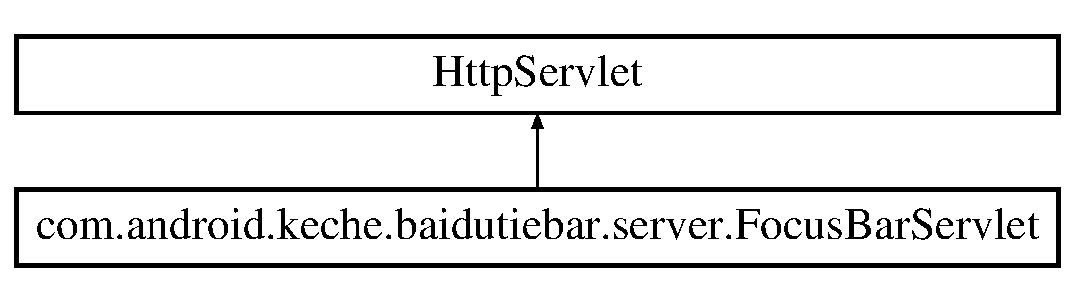
\includegraphics[height=2.000000cm]{classcom_1_1android_1_1keche_1_1baidutiebar_1_1server_1_1_focus_bar_servlet}
\end{center}
\end{figure}
\subsection*{Public 成员函数}
\begin{DoxyCompactItemize}
\item 
\mbox{\hyperlink{classcom_1_1android_1_1keche_1_1baidutiebar_1_1server_1_1_focus_bar_servlet_a80df07afce8969d2fba71a7998dec72c}{Focus\+Bar\+Servlet}} ()
\end{DoxyCompactItemize}
\subsection*{Protected 成员函数}
\begin{DoxyCompactItemize}
\item 
void \mbox{\hyperlink{classcom_1_1android_1_1keche_1_1baidutiebar_1_1server_1_1_focus_bar_servlet_aa0ab05484333a6f2e1825216ac79cc26}{do\+Get}} (Http\+Servlet\+Request request, Http\+Servlet\+Response response)  throws Servlet\+Exception, I\+O\+Exception 
\item 
void \mbox{\hyperlink{classcom_1_1android_1_1keche_1_1baidutiebar_1_1server_1_1_focus_bar_servlet_a1cb2ed55c3e4948ec9312e32379bd0ae}{do\+Post}} (Http\+Servlet\+Request request, Http\+Servlet\+Response response)  throws Servlet\+Exception, I\+O\+Exception 
\end{DoxyCompactItemize}


\subsection{详细描述}
Servlet implementation class \mbox{\hyperlink{classcom_1_1android_1_1keche_1_1baidutiebar_1_1server_1_1_focus_bar_servlet}{Focus\+Bar\+Servlet}} 

\subsection{构造及析构函数说明}
\mbox{\Hypertarget{classcom_1_1android_1_1keche_1_1baidutiebar_1_1server_1_1_focus_bar_servlet_a80df07afce8969d2fba71a7998dec72c}\label{classcom_1_1android_1_1keche_1_1baidutiebar_1_1server_1_1_focus_bar_servlet_a80df07afce8969d2fba71a7998dec72c}} 
\index{com\+::android\+::keche\+::baidutiebar\+::server\+::\+Focus\+Bar\+Servlet@{com\+::android\+::keche\+::baidutiebar\+::server\+::\+Focus\+Bar\+Servlet}!Focus\+Bar\+Servlet@{Focus\+Bar\+Servlet}}
\index{Focus\+Bar\+Servlet@{Focus\+Bar\+Servlet}!com\+::android\+::keche\+::baidutiebar\+::server\+::\+Focus\+Bar\+Servlet@{com\+::android\+::keche\+::baidutiebar\+::server\+::\+Focus\+Bar\+Servlet}}
\subsubsection{\texorpdfstring{Focus\+Bar\+Servlet()}{FocusBarServlet()}}
{\footnotesize\ttfamily com.\+android.\+keche.\+baidutiebar.\+server.\+Focus\+Bar\+Servlet.\+Focus\+Bar\+Servlet (\begin{DoxyParamCaption}{ }\end{DoxyParamCaption})\hspace{0.3cm}{\ttfamily [inline]}}

\begin{DoxySeeAlso}{参见}
Http\+Servlet\+::\+Http\+Servlet() 
\end{DoxySeeAlso}


\subsection{成员函数说明}
\mbox{\Hypertarget{classcom_1_1android_1_1keche_1_1baidutiebar_1_1server_1_1_focus_bar_servlet_aa0ab05484333a6f2e1825216ac79cc26}\label{classcom_1_1android_1_1keche_1_1baidutiebar_1_1server_1_1_focus_bar_servlet_aa0ab05484333a6f2e1825216ac79cc26}} 
\index{com\+::android\+::keche\+::baidutiebar\+::server\+::\+Focus\+Bar\+Servlet@{com\+::android\+::keche\+::baidutiebar\+::server\+::\+Focus\+Bar\+Servlet}!do\+Get@{do\+Get}}
\index{do\+Get@{do\+Get}!com\+::android\+::keche\+::baidutiebar\+::server\+::\+Focus\+Bar\+Servlet@{com\+::android\+::keche\+::baidutiebar\+::server\+::\+Focus\+Bar\+Servlet}}
\subsubsection{\texorpdfstring{do\+Get()}{doGet()}}
{\footnotesize\ttfamily void com.\+android.\+keche.\+baidutiebar.\+server.\+Focus\+Bar\+Servlet.\+do\+Get (\begin{DoxyParamCaption}\item[{Http\+Servlet\+Request}]{request,  }\item[{Http\+Servlet\+Response}]{response }\end{DoxyParamCaption}) throws Servlet\+Exception, I\+O\+Exception\hspace{0.3cm}{\ttfamily [inline]}, {\ttfamily [protected]}}

\begin{DoxySeeAlso}{参见}
Http\+Servlet\+::do\+Get(\+Http\+Servlet\+Request request, Http\+Servlet\+Response response) 
\end{DoxySeeAlso}
\mbox{\Hypertarget{classcom_1_1android_1_1keche_1_1baidutiebar_1_1server_1_1_focus_bar_servlet_a1cb2ed55c3e4948ec9312e32379bd0ae}\label{classcom_1_1android_1_1keche_1_1baidutiebar_1_1server_1_1_focus_bar_servlet_a1cb2ed55c3e4948ec9312e32379bd0ae}} 
\index{com\+::android\+::keche\+::baidutiebar\+::server\+::\+Focus\+Bar\+Servlet@{com\+::android\+::keche\+::baidutiebar\+::server\+::\+Focus\+Bar\+Servlet}!do\+Post@{do\+Post}}
\index{do\+Post@{do\+Post}!com\+::android\+::keche\+::baidutiebar\+::server\+::\+Focus\+Bar\+Servlet@{com\+::android\+::keche\+::baidutiebar\+::server\+::\+Focus\+Bar\+Servlet}}
\subsubsection{\texorpdfstring{do\+Post()}{doPost()}}
{\footnotesize\ttfamily void com.\+android.\+keche.\+baidutiebar.\+server.\+Focus\+Bar\+Servlet.\+do\+Post (\begin{DoxyParamCaption}\item[{Http\+Servlet\+Request}]{request,  }\item[{Http\+Servlet\+Response}]{response }\end{DoxyParamCaption}) throws Servlet\+Exception, I\+O\+Exception\hspace{0.3cm}{\ttfamily [inline]}, {\ttfamily [protected]}}

\begin{DoxySeeAlso}{参见}
Http\+Servlet\+::do\+Post(\+Http\+Servlet\+Request request, Http\+Servlet\+Response response) 
\end{DoxySeeAlso}


该类的文档由以下文件生成\+:\begin{DoxyCompactItemize}
\item 
src/com/android/keche/baidutiebar/server/Focus\+Bar\+Servlet.\+java\end{DoxyCompactItemize}

\hypertarget{classcom_1_1android_1_1keche_1_1baidutiebar_1_1server_1_1bean_1_1_focus_bean}{}\section{com.\+android.\+keche.\+baidutiebar.\+server.\+bean.\+Focus\+Bean类 参考}
\label{classcom_1_1android_1_1keche_1_1baidutiebar_1_1server_1_1bean_1_1_focus_bean}\index{com.\+android.\+keche.\+baidutiebar.\+server.\+bean.\+Focus\+Bean@{com.\+android.\+keche.\+baidutiebar.\+server.\+bean.\+Focus\+Bean}}
\subsection*{Public 成员函数}
\begin{DoxyCompactItemize}
\item 
\mbox{\Hypertarget{classcom_1_1android_1_1keche_1_1baidutiebar_1_1server_1_1bean_1_1_focus_bean_ab21d6e4febfdca9e080e4e8edbbf27db}\label{classcom_1_1android_1_1keche_1_1baidutiebar_1_1server_1_1bean_1_1_focus_bean_ab21d6e4febfdca9e080e4e8edbbf27db}} 
{\bfseries Focus\+Bean} (List$<$ String $>$ my\+Focu\+Text)
\item 
\mbox{\Hypertarget{classcom_1_1android_1_1keche_1_1baidutiebar_1_1server_1_1bean_1_1_focus_bean_adba1657ef08ed47f87eff0ee0880ad0f}\label{classcom_1_1android_1_1keche_1_1baidutiebar_1_1server_1_1bean_1_1_focus_bean_adba1657ef08ed47f87eff0ee0880ad0f}} 
List$<$ String $>$ {\bfseries get\+My\+Focu\+Text} ()
\item 
\mbox{\Hypertarget{classcom_1_1android_1_1keche_1_1baidutiebar_1_1server_1_1bean_1_1_focus_bean_a42ad9414f914ca93c28a020637c0f6b3}\label{classcom_1_1android_1_1keche_1_1baidutiebar_1_1server_1_1bean_1_1_focus_bean_a42ad9414f914ca93c28a020637c0f6b3}} 
void {\bfseries set\+My\+Focu\+Text} (List$<$ String $>$ my\+Focu\+Text)
\end{DoxyCompactItemize}


该类的文档由以下文件生成\+:\begin{DoxyCompactItemize}
\item 
src/com/android/keche/baidutiebar/server/bean/Focus\+Bean.\+java\end{DoxyCompactItemize}

\hypertarget{classcom_1_1android_1_1keche_1_1baidutiebar_1_1server_1_1_gain_rand_sheet_servlet}{}\section{com.\+android.\+keche.\+baidutiebar.\+server.\+Gain\+Rand\+Sheet\+Servlet类 参考}
\label{classcom_1_1android_1_1keche_1_1baidutiebar_1_1server_1_1_gain_rand_sheet_servlet}\index{com.\+android.\+keche.\+baidutiebar.\+server.\+Gain\+Rand\+Sheet\+Servlet@{com.\+android.\+keche.\+baidutiebar.\+server.\+Gain\+Rand\+Sheet\+Servlet}}
类 com.\+android.\+keche.\+baidutiebar.\+server.\+Gain\+Rand\+Sheet\+Servlet 继承关系图\+:\begin{figure}[H]
\begin{center}
\leavevmode
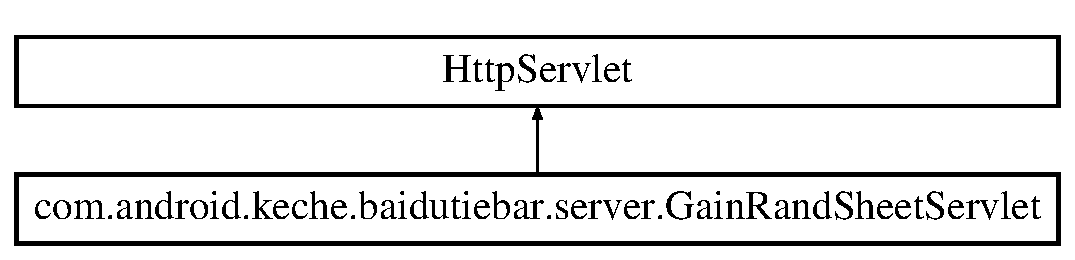
\includegraphics[height=2.000000cm]{classcom_1_1android_1_1keche_1_1baidutiebar_1_1server_1_1_gain_rand_sheet_servlet}
\end{center}
\end{figure}
\subsection*{Public 成员函数}
\begin{DoxyCompactItemize}
\item 
\mbox{\hyperlink{classcom_1_1android_1_1keche_1_1baidutiebar_1_1server_1_1_gain_rand_sheet_servlet_af71856b0ff809efcbf646987f01ad8e4}{Gain\+Rand\+Sheet\+Servlet}} ()
\end{DoxyCompactItemize}
\subsection*{Protected 成员函数}
\begin{DoxyCompactItemize}
\item 
void \mbox{\hyperlink{classcom_1_1android_1_1keche_1_1baidutiebar_1_1server_1_1_gain_rand_sheet_servlet_aac0f9b5813cd367ba330f249078a4441}{do\+Get}} (Http\+Servlet\+Request request, Http\+Servlet\+Response response)  throws Servlet\+Exception, I\+O\+Exception 
\item 
void \mbox{\hyperlink{classcom_1_1android_1_1keche_1_1baidutiebar_1_1server_1_1_gain_rand_sheet_servlet_accb367e2c96ba8ff2c86df33780d324b}{do\+Post}} (Http\+Servlet\+Request request, Http\+Servlet\+Response response)  throws Servlet\+Exception, I\+O\+Exception 
\end{DoxyCompactItemize}


\subsection{详细描述}
Servlet implementation class \mbox{\hyperlink{classcom_1_1android_1_1keche_1_1baidutiebar_1_1server_1_1_gain_rand_sheet_servlet}{Gain\+Rand\+Sheet\+Servlet}} 

\subsection{构造及析构函数说明}
\mbox{\Hypertarget{classcom_1_1android_1_1keche_1_1baidutiebar_1_1server_1_1_gain_rand_sheet_servlet_af71856b0ff809efcbf646987f01ad8e4}\label{classcom_1_1android_1_1keche_1_1baidutiebar_1_1server_1_1_gain_rand_sheet_servlet_af71856b0ff809efcbf646987f01ad8e4}} 
\index{com\+::android\+::keche\+::baidutiebar\+::server\+::\+Gain\+Rand\+Sheet\+Servlet@{com\+::android\+::keche\+::baidutiebar\+::server\+::\+Gain\+Rand\+Sheet\+Servlet}!Gain\+Rand\+Sheet\+Servlet@{Gain\+Rand\+Sheet\+Servlet}}
\index{Gain\+Rand\+Sheet\+Servlet@{Gain\+Rand\+Sheet\+Servlet}!com\+::android\+::keche\+::baidutiebar\+::server\+::\+Gain\+Rand\+Sheet\+Servlet@{com\+::android\+::keche\+::baidutiebar\+::server\+::\+Gain\+Rand\+Sheet\+Servlet}}
\subsubsection{\texorpdfstring{Gain\+Rand\+Sheet\+Servlet()}{GainRandSheetServlet()}}
{\footnotesize\ttfamily com.\+android.\+keche.\+baidutiebar.\+server.\+Gain\+Rand\+Sheet\+Servlet.\+Gain\+Rand\+Sheet\+Servlet (\begin{DoxyParamCaption}{ }\end{DoxyParamCaption})\hspace{0.3cm}{\ttfamily [inline]}}

\begin{DoxySeeAlso}{参见}
Http\+Servlet\+::\+Http\+Servlet() 
\end{DoxySeeAlso}


\subsection{成员函数说明}
\mbox{\Hypertarget{classcom_1_1android_1_1keche_1_1baidutiebar_1_1server_1_1_gain_rand_sheet_servlet_aac0f9b5813cd367ba330f249078a4441}\label{classcom_1_1android_1_1keche_1_1baidutiebar_1_1server_1_1_gain_rand_sheet_servlet_aac0f9b5813cd367ba330f249078a4441}} 
\index{com\+::android\+::keche\+::baidutiebar\+::server\+::\+Gain\+Rand\+Sheet\+Servlet@{com\+::android\+::keche\+::baidutiebar\+::server\+::\+Gain\+Rand\+Sheet\+Servlet}!do\+Get@{do\+Get}}
\index{do\+Get@{do\+Get}!com\+::android\+::keche\+::baidutiebar\+::server\+::\+Gain\+Rand\+Sheet\+Servlet@{com\+::android\+::keche\+::baidutiebar\+::server\+::\+Gain\+Rand\+Sheet\+Servlet}}
\subsubsection{\texorpdfstring{do\+Get()}{doGet()}}
{\footnotesize\ttfamily void com.\+android.\+keche.\+baidutiebar.\+server.\+Gain\+Rand\+Sheet\+Servlet.\+do\+Get (\begin{DoxyParamCaption}\item[{Http\+Servlet\+Request}]{request,  }\item[{Http\+Servlet\+Response}]{response }\end{DoxyParamCaption}) throws Servlet\+Exception, I\+O\+Exception\hspace{0.3cm}{\ttfamily [inline]}, {\ttfamily [protected]}}

\begin{DoxySeeAlso}{参见}
Http\+Servlet\+::do\+Get(\+Http\+Servlet\+Request request, Http\+Servlet\+Response response) 
\end{DoxySeeAlso}
\mbox{\Hypertarget{classcom_1_1android_1_1keche_1_1baidutiebar_1_1server_1_1_gain_rand_sheet_servlet_accb367e2c96ba8ff2c86df33780d324b}\label{classcom_1_1android_1_1keche_1_1baidutiebar_1_1server_1_1_gain_rand_sheet_servlet_accb367e2c96ba8ff2c86df33780d324b}} 
\index{com\+::android\+::keche\+::baidutiebar\+::server\+::\+Gain\+Rand\+Sheet\+Servlet@{com\+::android\+::keche\+::baidutiebar\+::server\+::\+Gain\+Rand\+Sheet\+Servlet}!do\+Post@{do\+Post}}
\index{do\+Post@{do\+Post}!com\+::android\+::keche\+::baidutiebar\+::server\+::\+Gain\+Rand\+Sheet\+Servlet@{com\+::android\+::keche\+::baidutiebar\+::server\+::\+Gain\+Rand\+Sheet\+Servlet}}
\subsubsection{\texorpdfstring{do\+Post()}{doPost()}}
{\footnotesize\ttfamily void com.\+android.\+keche.\+baidutiebar.\+server.\+Gain\+Rand\+Sheet\+Servlet.\+do\+Post (\begin{DoxyParamCaption}\item[{Http\+Servlet\+Request}]{request,  }\item[{Http\+Servlet\+Response}]{response }\end{DoxyParamCaption}) throws Servlet\+Exception, I\+O\+Exception\hspace{0.3cm}{\ttfamily [inline]}, {\ttfamily [protected]}}

\begin{DoxySeeAlso}{参见}
Http\+Servlet\+::do\+Post(\+Http\+Servlet\+Request request, Http\+Servlet\+Response response) 
\end{DoxySeeAlso}


该类的文档由以下文件生成\+:\begin{DoxyCompactItemize}
\item 
src/com/android/keche/baidutiebar/server/Gain\+Rand\+Sheet\+Servlet.\+java\end{DoxyCompactItemize}

\hypertarget{classcom_1_1android_1_1keche_1_1baidutiebar_1_1server_1_1bean_1_1_group_bean}{}\section{com.\+android.\+keche.\+baidutiebar.\+server.\+bean.\+Group\+Bean类 参考}
\label{classcom_1_1android_1_1keche_1_1baidutiebar_1_1server_1_1bean_1_1_group_bean}\index{com.\+android.\+keche.\+baidutiebar.\+server.\+bean.\+Group\+Bean@{com.\+android.\+keche.\+baidutiebar.\+server.\+bean.\+Group\+Bean}}
\subsection*{Public 成员函数}
\begin{DoxyCompactItemize}
\item 
\mbox{\Hypertarget{classcom_1_1android_1_1keche_1_1baidutiebar_1_1server_1_1bean_1_1_group_bean_a29ff414d1a7b9cf2e942da2c694aee2f}\label{classcom_1_1android_1_1keche_1_1baidutiebar_1_1server_1_1bean_1_1_group_bean_a29ff414d1a7b9cf2e942da2c694aee2f}} 
{\bfseries Group\+Bean} (String title, String source, String time)
\item 
\mbox{\Hypertarget{classcom_1_1android_1_1keche_1_1baidutiebar_1_1server_1_1bean_1_1_group_bean_a9005a28086e56f820c3ed5818d9d49cf}\label{classcom_1_1android_1_1keche_1_1baidutiebar_1_1server_1_1bean_1_1_group_bean_a9005a28086e56f820c3ed5818d9d49cf}} 
String {\bfseries get\+Title} ()
\item 
\mbox{\Hypertarget{classcom_1_1android_1_1keche_1_1baidutiebar_1_1server_1_1bean_1_1_group_bean_ae6a93af6b72e9d2c0661fe263f148aca}\label{classcom_1_1android_1_1keche_1_1baidutiebar_1_1server_1_1bean_1_1_group_bean_ae6a93af6b72e9d2c0661fe263f148aca}} 
void {\bfseries set\+Title} (String title)
\item 
\mbox{\Hypertarget{classcom_1_1android_1_1keche_1_1baidutiebar_1_1server_1_1bean_1_1_group_bean_a780ba7471be9a3c53fd1e8b9766e0a38}\label{classcom_1_1android_1_1keche_1_1baidutiebar_1_1server_1_1bean_1_1_group_bean_a780ba7471be9a3c53fd1e8b9766e0a38}} 
String {\bfseries get\+Source} ()
\item 
\mbox{\Hypertarget{classcom_1_1android_1_1keche_1_1baidutiebar_1_1server_1_1bean_1_1_group_bean_ab94c30822e9a3cccd2c3ac7893167dfb}\label{classcom_1_1android_1_1keche_1_1baidutiebar_1_1server_1_1bean_1_1_group_bean_ab94c30822e9a3cccd2c3ac7893167dfb}} 
void {\bfseries set\+Source} (String source)
\item 
\mbox{\Hypertarget{classcom_1_1android_1_1keche_1_1baidutiebar_1_1server_1_1bean_1_1_group_bean_a9280df18ab3ae1cdd5266ee9e32e9d6d}\label{classcom_1_1android_1_1keche_1_1baidutiebar_1_1server_1_1bean_1_1_group_bean_a9280df18ab3ae1cdd5266ee9e32e9d6d}} 
String {\bfseries get\+Time} ()
\item 
\mbox{\Hypertarget{classcom_1_1android_1_1keche_1_1baidutiebar_1_1server_1_1bean_1_1_group_bean_a5507bf6820306e8e5f06541739284b90}\label{classcom_1_1android_1_1keche_1_1baidutiebar_1_1server_1_1bean_1_1_group_bean_a5507bf6820306e8e5f06541739284b90}} 
void {\bfseries set\+Time} (String time)
\end{DoxyCompactItemize}


该类的文档由以下文件生成\+:\begin{DoxyCompactItemize}
\item 
src/com/android/keche/baidutiebar/server/bean/Group\+Bean.\+java\end{DoxyCompactItemize}

\hypertarget{classcom_1_1android_1_1keche_1_1baidutiebar_1_1server_1_1_group_servlet}{}\section{com.\+android.\+keche.\+baidutiebar.\+server.\+Group\+Servlet类 参考}
\label{classcom_1_1android_1_1keche_1_1baidutiebar_1_1server_1_1_group_servlet}\index{com.\+android.\+keche.\+baidutiebar.\+server.\+Group\+Servlet@{com.\+android.\+keche.\+baidutiebar.\+server.\+Group\+Servlet}}
类 com.\+android.\+keche.\+baidutiebar.\+server.\+Group\+Servlet 继承关系图\+:\begin{figure}[H]
\begin{center}
\leavevmode
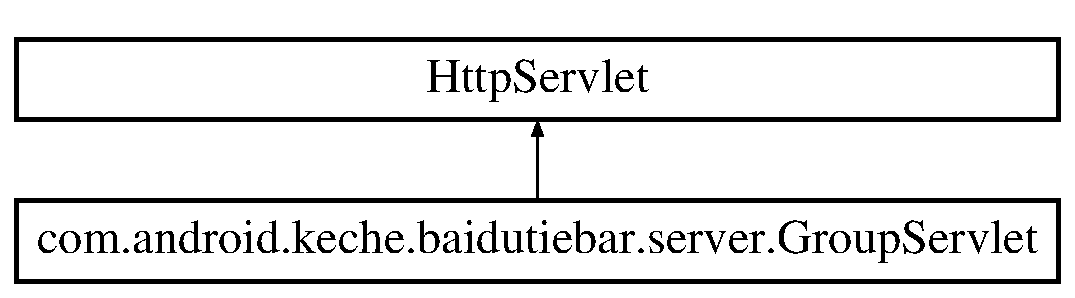
\includegraphics[height=2.000000cm]{classcom_1_1android_1_1keche_1_1baidutiebar_1_1server_1_1_group_servlet}
\end{center}
\end{figure}
\subsection*{Public 成员函数}
\begin{DoxyCompactItemize}
\item 
\mbox{\hyperlink{classcom_1_1android_1_1keche_1_1baidutiebar_1_1server_1_1_group_servlet_afe9741000f3e3939a050be653dcdfea6}{Group\+Servlet}} ()
\end{DoxyCompactItemize}
\subsection*{Protected 成员函数}
\begin{DoxyCompactItemize}
\item 
void \mbox{\hyperlink{classcom_1_1android_1_1keche_1_1baidutiebar_1_1server_1_1_group_servlet_ad037d3fc8d03e2c707d34e17fa8bf49b}{do\+Get}} (Http\+Servlet\+Request request, Http\+Servlet\+Response response)  throws Servlet\+Exception, I\+O\+Exception 
\item 
void \mbox{\hyperlink{classcom_1_1android_1_1keche_1_1baidutiebar_1_1server_1_1_group_servlet_aa9b08b4da3a8fde05198fa1e6aec01ca}{do\+Post}} (Http\+Servlet\+Request request, Http\+Servlet\+Response response)  throws Servlet\+Exception, I\+O\+Exception 
\end{DoxyCompactItemize}


\subsection{详细描述}
Servlet implementation class \mbox{\hyperlink{classcom_1_1android_1_1keche_1_1baidutiebar_1_1server_1_1_group_servlet}{Group\+Servlet}} 

\subsection{构造及析构函数说明}
\mbox{\Hypertarget{classcom_1_1android_1_1keche_1_1baidutiebar_1_1server_1_1_group_servlet_afe9741000f3e3939a050be653dcdfea6}\label{classcom_1_1android_1_1keche_1_1baidutiebar_1_1server_1_1_group_servlet_afe9741000f3e3939a050be653dcdfea6}} 
\index{com\+::android\+::keche\+::baidutiebar\+::server\+::\+Group\+Servlet@{com\+::android\+::keche\+::baidutiebar\+::server\+::\+Group\+Servlet}!Group\+Servlet@{Group\+Servlet}}
\index{Group\+Servlet@{Group\+Servlet}!com\+::android\+::keche\+::baidutiebar\+::server\+::\+Group\+Servlet@{com\+::android\+::keche\+::baidutiebar\+::server\+::\+Group\+Servlet}}
\subsubsection{\texorpdfstring{Group\+Servlet()}{GroupServlet()}}
{\footnotesize\ttfamily com.\+android.\+keche.\+baidutiebar.\+server.\+Group\+Servlet.\+Group\+Servlet (\begin{DoxyParamCaption}{ }\end{DoxyParamCaption})\hspace{0.3cm}{\ttfamily [inline]}}

\begin{DoxySeeAlso}{参见}
Http\+Servlet\+::\+Http\+Servlet() 
\end{DoxySeeAlso}


\subsection{成员函数说明}
\mbox{\Hypertarget{classcom_1_1android_1_1keche_1_1baidutiebar_1_1server_1_1_group_servlet_ad037d3fc8d03e2c707d34e17fa8bf49b}\label{classcom_1_1android_1_1keche_1_1baidutiebar_1_1server_1_1_group_servlet_ad037d3fc8d03e2c707d34e17fa8bf49b}} 
\index{com\+::android\+::keche\+::baidutiebar\+::server\+::\+Group\+Servlet@{com\+::android\+::keche\+::baidutiebar\+::server\+::\+Group\+Servlet}!do\+Get@{do\+Get}}
\index{do\+Get@{do\+Get}!com\+::android\+::keche\+::baidutiebar\+::server\+::\+Group\+Servlet@{com\+::android\+::keche\+::baidutiebar\+::server\+::\+Group\+Servlet}}
\subsubsection{\texorpdfstring{do\+Get()}{doGet()}}
{\footnotesize\ttfamily void com.\+android.\+keche.\+baidutiebar.\+server.\+Group\+Servlet.\+do\+Get (\begin{DoxyParamCaption}\item[{Http\+Servlet\+Request}]{request,  }\item[{Http\+Servlet\+Response}]{response }\end{DoxyParamCaption}) throws Servlet\+Exception, I\+O\+Exception\hspace{0.3cm}{\ttfamily [inline]}, {\ttfamily [protected]}}

\begin{DoxySeeAlso}{参见}
Http\+Servlet\+::do\+Get(\+Http\+Servlet\+Request request, Http\+Servlet\+Response response) 
\end{DoxySeeAlso}
\mbox{\Hypertarget{classcom_1_1android_1_1keche_1_1baidutiebar_1_1server_1_1_group_servlet_aa9b08b4da3a8fde05198fa1e6aec01ca}\label{classcom_1_1android_1_1keche_1_1baidutiebar_1_1server_1_1_group_servlet_aa9b08b4da3a8fde05198fa1e6aec01ca}} 
\index{com\+::android\+::keche\+::baidutiebar\+::server\+::\+Group\+Servlet@{com\+::android\+::keche\+::baidutiebar\+::server\+::\+Group\+Servlet}!do\+Post@{do\+Post}}
\index{do\+Post@{do\+Post}!com\+::android\+::keche\+::baidutiebar\+::server\+::\+Group\+Servlet@{com\+::android\+::keche\+::baidutiebar\+::server\+::\+Group\+Servlet}}
\subsubsection{\texorpdfstring{do\+Post()}{doPost()}}
{\footnotesize\ttfamily void com.\+android.\+keche.\+baidutiebar.\+server.\+Group\+Servlet.\+do\+Post (\begin{DoxyParamCaption}\item[{Http\+Servlet\+Request}]{request,  }\item[{Http\+Servlet\+Response}]{response }\end{DoxyParamCaption}) throws Servlet\+Exception, I\+O\+Exception\hspace{0.3cm}{\ttfamily [inline]}, {\ttfamily [protected]}}

\begin{DoxySeeAlso}{参见}
Http\+Servlet\+::do\+Post(\+Http\+Servlet\+Request request, Http\+Servlet\+Response response) 
\end{DoxySeeAlso}


该类的文档由以下文件生成\+:\begin{DoxyCompactItemize}
\item 
src/com/android/keche/baidutiebar/server/Group\+Servlet.\+java\end{DoxyCompactItemize}

\hypertarget{classcom_1_1android_1_1keche_1_1baidutiebar_1_1server_1_1bean_1_1_history_bean}{}\section{com.\+android.\+keche.\+baidutiebar.\+server.\+bean.\+History\+Bean类 参考}
\label{classcom_1_1android_1_1keche_1_1baidutiebar_1_1server_1_1bean_1_1_history_bean}\index{com.\+android.\+keche.\+baidutiebar.\+server.\+bean.\+History\+Bean@{com.\+android.\+keche.\+baidutiebar.\+server.\+bean.\+History\+Bean}}
\subsection*{Public 成员函数}
\begin{DoxyCompactItemize}
\item 
\mbox{\Hypertarget{classcom_1_1android_1_1keche_1_1baidutiebar_1_1server_1_1bean_1_1_history_bean_a3e26dd4e6369e2564de4675a1a8baa4d}\label{classcom_1_1android_1_1keche_1_1baidutiebar_1_1server_1_1bean_1_1_history_bean_a3e26dd4e6369e2564de4675a1a8baa4d}} 
{\bfseries History\+Bean} (String title, String source, String time)
\item 
\mbox{\Hypertarget{classcom_1_1android_1_1keche_1_1baidutiebar_1_1server_1_1bean_1_1_history_bean_a4c53786442e14dffef3c29269289b44f}\label{classcom_1_1android_1_1keche_1_1baidutiebar_1_1server_1_1bean_1_1_history_bean_a4c53786442e14dffef3c29269289b44f}} 
String {\bfseries get\+Title} ()
\item 
\mbox{\Hypertarget{classcom_1_1android_1_1keche_1_1baidutiebar_1_1server_1_1bean_1_1_history_bean_a710912318668039881c80cdee9dd4b5c}\label{classcom_1_1android_1_1keche_1_1baidutiebar_1_1server_1_1bean_1_1_history_bean_a710912318668039881c80cdee9dd4b5c}} 
void {\bfseries set\+Title} (String title)
\item 
\mbox{\Hypertarget{classcom_1_1android_1_1keche_1_1baidutiebar_1_1server_1_1bean_1_1_history_bean_ac2242c477e7b2a1946476b6f28000573}\label{classcom_1_1android_1_1keche_1_1baidutiebar_1_1server_1_1bean_1_1_history_bean_ac2242c477e7b2a1946476b6f28000573}} 
String {\bfseries get\+Source} ()
\item 
\mbox{\Hypertarget{classcom_1_1android_1_1keche_1_1baidutiebar_1_1server_1_1bean_1_1_history_bean_a4b6baf6a05fcfd81372e093ed460034f}\label{classcom_1_1android_1_1keche_1_1baidutiebar_1_1server_1_1bean_1_1_history_bean_a4b6baf6a05fcfd81372e093ed460034f}} 
void {\bfseries set\+Source} (String source)
\item 
\mbox{\Hypertarget{classcom_1_1android_1_1keche_1_1baidutiebar_1_1server_1_1bean_1_1_history_bean_aa0a5e52d86980c42ea85b3efd4f77b73}\label{classcom_1_1android_1_1keche_1_1baidutiebar_1_1server_1_1bean_1_1_history_bean_aa0a5e52d86980c42ea85b3efd4f77b73}} 
String {\bfseries get\+Time} ()
\item 
\mbox{\Hypertarget{classcom_1_1android_1_1keche_1_1baidutiebar_1_1server_1_1bean_1_1_history_bean_a61171edddb8ea4f00837415bdf187034}\label{classcom_1_1android_1_1keche_1_1baidutiebar_1_1server_1_1bean_1_1_history_bean_a61171edddb8ea4f00837415bdf187034}} 
void {\bfseries set\+Time} (String time)
\end{DoxyCompactItemize}


该类的文档由以下文件生成\+:\begin{DoxyCompactItemize}
\item 
src/com/android/keche/baidutiebar/server/bean/History\+Bean.\+java\end{DoxyCompactItemize}

\hypertarget{classcom_1_1android_1_1keche_1_1baidutiebar_1_1server_1_1_history_servlet}{}\section{com.\+android.\+keche.\+baidutiebar.\+server.\+History\+Servlet类 参考}
\label{classcom_1_1android_1_1keche_1_1baidutiebar_1_1server_1_1_history_servlet}\index{com.\+android.\+keche.\+baidutiebar.\+server.\+History\+Servlet@{com.\+android.\+keche.\+baidutiebar.\+server.\+History\+Servlet}}
类 com.\+android.\+keche.\+baidutiebar.\+server.\+History\+Servlet 继承关系图\+:\begin{figure}[H]
\begin{center}
\leavevmode
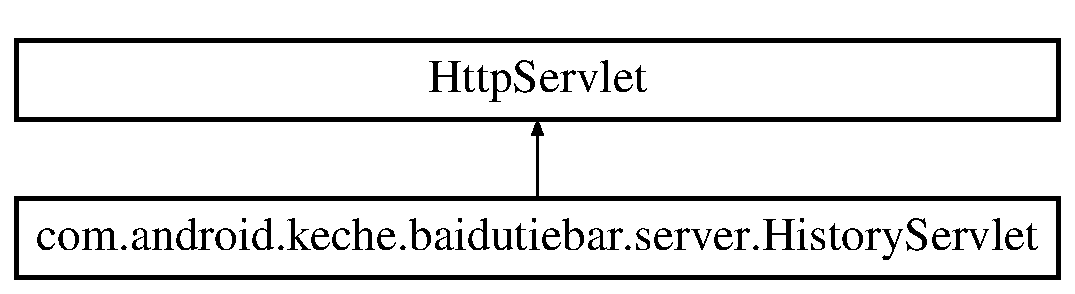
\includegraphics[height=2.000000cm]{classcom_1_1android_1_1keche_1_1baidutiebar_1_1server_1_1_history_servlet}
\end{center}
\end{figure}
\subsection*{Public 成员函数}
\begin{DoxyCompactItemize}
\item 
\mbox{\hyperlink{classcom_1_1android_1_1keche_1_1baidutiebar_1_1server_1_1_history_servlet_a1ad77d9d8e390da15db2f9fc756d2880}{History\+Servlet}} ()
\end{DoxyCompactItemize}
\subsection*{Protected 成员函数}
\begin{DoxyCompactItemize}
\item 
void \mbox{\hyperlink{classcom_1_1android_1_1keche_1_1baidutiebar_1_1server_1_1_history_servlet_a27515d01f2660e911b8d176bee1541ea}{do\+Get}} (Http\+Servlet\+Request request, Http\+Servlet\+Response response)  throws Servlet\+Exception, I\+O\+Exception 
\item 
void \mbox{\hyperlink{classcom_1_1android_1_1keche_1_1baidutiebar_1_1server_1_1_history_servlet_aa5f065d950c5794b099a4106592862b5}{do\+Post}} (Http\+Servlet\+Request request, Http\+Servlet\+Response response)  throws Servlet\+Exception, I\+O\+Exception 
\end{DoxyCompactItemize}


\subsection{详细描述}
Servlet implementation class \mbox{\hyperlink{classcom_1_1android_1_1keche_1_1baidutiebar_1_1server_1_1_history_servlet}{History\+Servlet}} 

\subsection{构造及析构函数说明}
\mbox{\Hypertarget{classcom_1_1android_1_1keche_1_1baidutiebar_1_1server_1_1_history_servlet_a1ad77d9d8e390da15db2f9fc756d2880}\label{classcom_1_1android_1_1keche_1_1baidutiebar_1_1server_1_1_history_servlet_a1ad77d9d8e390da15db2f9fc756d2880}} 
\index{com\+::android\+::keche\+::baidutiebar\+::server\+::\+History\+Servlet@{com\+::android\+::keche\+::baidutiebar\+::server\+::\+History\+Servlet}!History\+Servlet@{History\+Servlet}}
\index{History\+Servlet@{History\+Servlet}!com\+::android\+::keche\+::baidutiebar\+::server\+::\+History\+Servlet@{com\+::android\+::keche\+::baidutiebar\+::server\+::\+History\+Servlet}}
\subsubsection{\texorpdfstring{History\+Servlet()}{HistoryServlet()}}
{\footnotesize\ttfamily com.\+android.\+keche.\+baidutiebar.\+server.\+History\+Servlet.\+History\+Servlet (\begin{DoxyParamCaption}{ }\end{DoxyParamCaption})\hspace{0.3cm}{\ttfamily [inline]}}

\begin{DoxySeeAlso}{参见}
Http\+Servlet\+::\+Http\+Servlet() 
\end{DoxySeeAlso}


\subsection{成员函数说明}
\mbox{\Hypertarget{classcom_1_1android_1_1keche_1_1baidutiebar_1_1server_1_1_history_servlet_a27515d01f2660e911b8d176bee1541ea}\label{classcom_1_1android_1_1keche_1_1baidutiebar_1_1server_1_1_history_servlet_a27515d01f2660e911b8d176bee1541ea}} 
\index{com\+::android\+::keche\+::baidutiebar\+::server\+::\+History\+Servlet@{com\+::android\+::keche\+::baidutiebar\+::server\+::\+History\+Servlet}!do\+Get@{do\+Get}}
\index{do\+Get@{do\+Get}!com\+::android\+::keche\+::baidutiebar\+::server\+::\+History\+Servlet@{com\+::android\+::keche\+::baidutiebar\+::server\+::\+History\+Servlet}}
\subsubsection{\texorpdfstring{do\+Get()}{doGet()}}
{\footnotesize\ttfamily void com.\+android.\+keche.\+baidutiebar.\+server.\+History\+Servlet.\+do\+Get (\begin{DoxyParamCaption}\item[{Http\+Servlet\+Request}]{request,  }\item[{Http\+Servlet\+Response}]{response }\end{DoxyParamCaption}) throws Servlet\+Exception, I\+O\+Exception\hspace{0.3cm}{\ttfamily [inline]}, {\ttfamily [protected]}}

\begin{DoxySeeAlso}{参见}
Http\+Servlet\+::do\+Get(\+Http\+Servlet\+Request request, Http\+Servlet\+Response response) 
\end{DoxySeeAlso}
\mbox{\Hypertarget{classcom_1_1android_1_1keche_1_1baidutiebar_1_1server_1_1_history_servlet_aa5f065d950c5794b099a4106592862b5}\label{classcom_1_1android_1_1keche_1_1baidutiebar_1_1server_1_1_history_servlet_aa5f065d950c5794b099a4106592862b5}} 
\index{com\+::android\+::keche\+::baidutiebar\+::server\+::\+History\+Servlet@{com\+::android\+::keche\+::baidutiebar\+::server\+::\+History\+Servlet}!do\+Post@{do\+Post}}
\index{do\+Post@{do\+Post}!com\+::android\+::keche\+::baidutiebar\+::server\+::\+History\+Servlet@{com\+::android\+::keche\+::baidutiebar\+::server\+::\+History\+Servlet}}
\subsubsection{\texorpdfstring{do\+Post()}{doPost()}}
{\footnotesize\ttfamily void com.\+android.\+keche.\+baidutiebar.\+server.\+History\+Servlet.\+do\+Post (\begin{DoxyParamCaption}\item[{Http\+Servlet\+Request}]{request,  }\item[{Http\+Servlet\+Response}]{response }\end{DoxyParamCaption}) throws Servlet\+Exception, I\+O\+Exception\hspace{0.3cm}{\ttfamily [inline]}, {\ttfamily [protected]}}

\begin{DoxySeeAlso}{参见}
Http\+Servlet\+::do\+Post(\+Http\+Servlet\+Request request, Http\+Servlet\+Response response) 
\end{DoxySeeAlso}


该类的文档由以下文件生成\+:\begin{DoxyCompactItemize}
\item 
src/com/android/keche/baidutiebar/server/History\+Servlet.\+java\end{DoxyCompactItemize}

\hypertarget{classcom_1_1android_1_1keche_1_1baidutiebar_1_1server_1_1_insert_sheet_servlet}{}\section{com.\+android.\+keche.\+baidutiebar.\+server.\+Insert\+Sheet\+Servlet类 参考}
\label{classcom_1_1android_1_1keche_1_1baidutiebar_1_1server_1_1_insert_sheet_servlet}\index{com.\+android.\+keche.\+baidutiebar.\+server.\+Insert\+Sheet\+Servlet@{com.\+android.\+keche.\+baidutiebar.\+server.\+Insert\+Sheet\+Servlet}}
类 com.\+android.\+keche.\+baidutiebar.\+server.\+Insert\+Sheet\+Servlet 继承关系图\+:\begin{figure}[H]
\begin{center}
\leavevmode
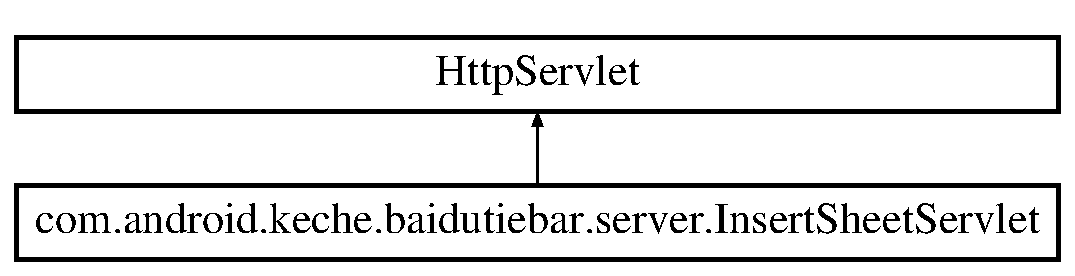
\includegraphics[height=2.000000cm]{classcom_1_1android_1_1keche_1_1baidutiebar_1_1server_1_1_insert_sheet_servlet}
\end{center}
\end{figure}
\subsection*{Public 成员函数}
\begin{DoxyCompactItemize}
\item 
\mbox{\hyperlink{classcom_1_1android_1_1keche_1_1baidutiebar_1_1server_1_1_insert_sheet_servlet_a948ff760e2d129d00a6420a48411d1df}{Insert\+Sheet\+Servlet}} ()
\end{DoxyCompactItemize}
\subsection*{Protected 成员函数}
\begin{DoxyCompactItemize}
\item 
void \mbox{\hyperlink{classcom_1_1android_1_1keche_1_1baidutiebar_1_1server_1_1_insert_sheet_servlet_a1719bd6108ece268a5bc4ae2f99ba696}{do\+Get}} (Http\+Servlet\+Request request, Http\+Servlet\+Response response)  throws Servlet\+Exception, I\+O\+Exception 
\item 
void \mbox{\hyperlink{classcom_1_1android_1_1keche_1_1baidutiebar_1_1server_1_1_insert_sheet_servlet_afda7ec1d201f7ace619c57faa3e36a8e}{do\+Post}} (Http\+Servlet\+Request request, Http\+Servlet\+Response response)  throws Servlet\+Exception, I\+O\+Exception 
\end{DoxyCompactItemize}


\subsection{详细描述}
Servlet implementation class \mbox{\hyperlink{classcom_1_1android_1_1keche_1_1baidutiebar_1_1server_1_1_insert_sheet_servlet}{Insert\+Sheet\+Servlet}} 

\subsection{构造及析构函数说明}
\mbox{\Hypertarget{classcom_1_1android_1_1keche_1_1baidutiebar_1_1server_1_1_insert_sheet_servlet_a948ff760e2d129d00a6420a48411d1df}\label{classcom_1_1android_1_1keche_1_1baidutiebar_1_1server_1_1_insert_sheet_servlet_a948ff760e2d129d00a6420a48411d1df}} 
\index{com\+::android\+::keche\+::baidutiebar\+::server\+::\+Insert\+Sheet\+Servlet@{com\+::android\+::keche\+::baidutiebar\+::server\+::\+Insert\+Sheet\+Servlet}!Insert\+Sheet\+Servlet@{Insert\+Sheet\+Servlet}}
\index{Insert\+Sheet\+Servlet@{Insert\+Sheet\+Servlet}!com\+::android\+::keche\+::baidutiebar\+::server\+::\+Insert\+Sheet\+Servlet@{com\+::android\+::keche\+::baidutiebar\+::server\+::\+Insert\+Sheet\+Servlet}}
\subsubsection{\texorpdfstring{Insert\+Sheet\+Servlet()}{InsertSheetServlet()}}
{\footnotesize\ttfamily com.\+android.\+keche.\+baidutiebar.\+server.\+Insert\+Sheet\+Servlet.\+Insert\+Sheet\+Servlet (\begin{DoxyParamCaption}{ }\end{DoxyParamCaption})\hspace{0.3cm}{\ttfamily [inline]}}

\begin{DoxySeeAlso}{参见}
Http\+Servlet\+::\+Http\+Servlet() 
\end{DoxySeeAlso}


\subsection{成员函数说明}
\mbox{\Hypertarget{classcom_1_1android_1_1keche_1_1baidutiebar_1_1server_1_1_insert_sheet_servlet_a1719bd6108ece268a5bc4ae2f99ba696}\label{classcom_1_1android_1_1keche_1_1baidutiebar_1_1server_1_1_insert_sheet_servlet_a1719bd6108ece268a5bc4ae2f99ba696}} 
\index{com\+::android\+::keche\+::baidutiebar\+::server\+::\+Insert\+Sheet\+Servlet@{com\+::android\+::keche\+::baidutiebar\+::server\+::\+Insert\+Sheet\+Servlet}!do\+Get@{do\+Get}}
\index{do\+Get@{do\+Get}!com\+::android\+::keche\+::baidutiebar\+::server\+::\+Insert\+Sheet\+Servlet@{com\+::android\+::keche\+::baidutiebar\+::server\+::\+Insert\+Sheet\+Servlet}}
\subsubsection{\texorpdfstring{do\+Get()}{doGet()}}
{\footnotesize\ttfamily void com.\+android.\+keche.\+baidutiebar.\+server.\+Insert\+Sheet\+Servlet.\+do\+Get (\begin{DoxyParamCaption}\item[{Http\+Servlet\+Request}]{request,  }\item[{Http\+Servlet\+Response}]{response }\end{DoxyParamCaption}) throws Servlet\+Exception, I\+O\+Exception\hspace{0.3cm}{\ttfamily [inline]}, {\ttfamily [protected]}}

\begin{DoxySeeAlso}{参见}
Http\+Servlet\+::do\+Get(\+Http\+Servlet\+Request request, Http\+Servlet\+Response response) 
\end{DoxySeeAlso}
\mbox{\Hypertarget{classcom_1_1android_1_1keche_1_1baidutiebar_1_1server_1_1_insert_sheet_servlet_afda7ec1d201f7ace619c57faa3e36a8e}\label{classcom_1_1android_1_1keche_1_1baidutiebar_1_1server_1_1_insert_sheet_servlet_afda7ec1d201f7ace619c57faa3e36a8e}} 
\index{com\+::android\+::keche\+::baidutiebar\+::server\+::\+Insert\+Sheet\+Servlet@{com\+::android\+::keche\+::baidutiebar\+::server\+::\+Insert\+Sheet\+Servlet}!do\+Post@{do\+Post}}
\index{do\+Post@{do\+Post}!com\+::android\+::keche\+::baidutiebar\+::server\+::\+Insert\+Sheet\+Servlet@{com\+::android\+::keche\+::baidutiebar\+::server\+::\+Insert\+Sheet\+Servlet}}
\subsubsection{\texorpdfstring{do\+Post()}{doPost()}}
{\footnotesize\ttfamily void com.\+android.\+keche.\+baidutiebar.\+server.\+Insert\+Sheet\+Servlet.\+do\+Post (\begin{DoxyParamCaption}\item[{Http\+Servlet\+Request}]{request,  }\item[{Http\+Servlet\+Response}]{response }\end{DoxyParamCaption}) throws Servlet\+Exception, I\+O\+Exception\hspace{0.3cm}{\ttfamily [inline]}, {\ttfamily [protected]}}

\begin{DoxySeeAlso}{参见}
Http\+Servlet\+::do\+Post(\+Http\+Servlet\+Request request, Http\+Servlet\+Response response) 
\end{DoxySeeAlso}


该类的文档由以下文件生成\+:\begin{DoxyCompactItemize}
\item 
src/com/android/keche/baidutiebar/server/Insert\+Sheet\+Servlet.\+java\end{DoxyCompactItemize}

\hypertarget{classcom_1_1android_1_1keche_1_1baidutiebar_1_1server_1_1_message_servlet}{}\section{com.\+android.\+keche.\+baidutiebar.\+server.\+Message\+Servlet类 参考}
\label{classcom_1_1android_1_1keche_1_1baidutiebar_1_1server_1_1_message_servlet}\index{com.\+android.\+keche.\+baidutiebar.\+server.\+Message\+Servlet@{com.\+android.\+keche.\+baidutiebar.\+server.\+Message\+Servlet}}
类 com.\+android.\+keche.\+baidutiebar.\+server.\+Message\+Servlet 继承关系图\+:\begin{figure}[H]
\begin{center}
\leavevmode
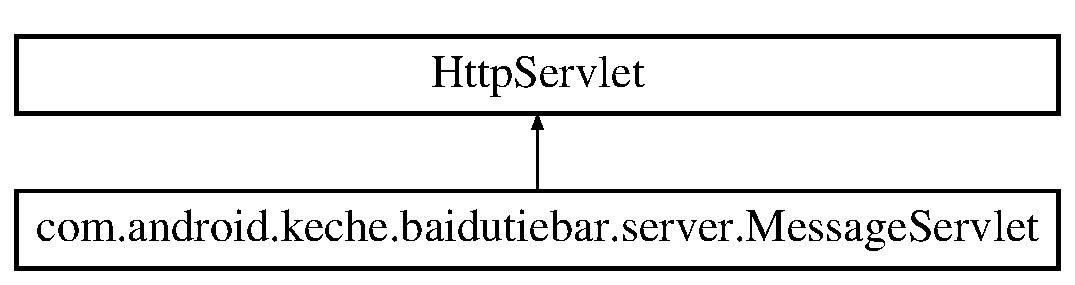
\includegraphics[height=2.000000cm]{classcom_1_1android_1_1keche_1_1baidutiebar_1_1server_1_1_message_servlet}
\end{center}
\end{figure}
\subsection*{Public 成员函数}
\begin{DoxyCompactItemize}
\item 
\mbox{\hyperlink{classcom_1_1android_1_1keche_1_1baidutiebar_1_1server_1_1_message_servlet_aef435c6cd6a902c4509080864a588bad}{Message\+Servlet}} ()
\end{DoxyCompactItemize}
\subsection*{Protected 成员函数}
\begin{DoxyCompactItemize}
\item 
void \mbox{\hyperlink{classcom_1_1android_1_1keche_1_1baidutiebar_1_1server_1_1_message_servlet_a41a82e5e86882c5e69a120943f08f358}{do\+Get}} (Http\+Servlet\+Request request, Http\+Servlet\+Response response)  throws Servlet\+Exception, I\+O\+Exception 
\item 
void \mbox{\hyperlink{classcom_1_1android_1_1keche_1_1baidutiebar_1_1server_1_1_message_servlet_ae920f7609054c4ccff3a808c4e3ca9b0}{do\+Post}} (Http\+Servlet\+Request request, Http\+Servlet\+Response response)  throws Servlet\+Exception, I\+O\+Exception 
\end{DoxyCompactItemize}


\subsection{详细描述}
Servlet implementation class \mbox{\hyperlink{classcom_1_1android_1_1keche_1_1baidutiebar_1_1server_1_1_message_servlet}{Message\+Servlet}} 

\subsection{构造及析构函数说明}
\mbox{\Hypertarget{classcom_1_1android_1_1keche_1_1baidutiebar_1_1server_1_1_message_servlet_aef435c6cd6a902c4509080864a588bad}\label{classcom_1_1android_1_1keche_1_1baidutiebar_1_1server_1_1_message_servlet_aef435c6cd6a902c4509080864a588bad}} 
\index{com\+::android\+::keche\+::baidutiebar\+::server\+::\+Message\+Servlet@{com\+::android\+::keche\+::baidutiebar\+::server\+::\+Message\+Servlet}!Message\+Servlet@{Message\+Servlet}}
\index{Message\+Servlet@{Message\+Servlet}!com\+::android\+::keche\+::baidutiebar\+::server\+::\+Message\+Servlet@{com\+::android\+::keche\+::baidutiebar\+::server\+::\+Message\+Servlet}}
\subsubsection{\texorpdfstring{Message\+Servlet()}{MessageServlet()}}
{\footnotesize\ttfamily com.\+android.\+keche.\+baidutiebar.\+server.\+Message\+Servlet.\+Message\+Servlet (\begin{DoxyParamCaption}{ }\end{DoxyParamCaption})\hspace{0.3cm}{\ttfamily [inline]}}

\begin{DoxySeeAlso}{参见}
Http\+Servlet\+::\+Http\+Servlet() 
\end{DoxySeeAlso}


\subsection{成员函数说明}
\mbox{\Hypertarget{classcom_1_1android_1_1keche_1_1baidutiebar_1_1server_1_1_message_servlet_a41a82e5e86882c5e69a120943f08f358}\label{classcom_1_1android_1_1keche_1_1baidutiebar_1_1server_1_1_message_servlet_a41a82e5e86882c5e69a120943f08f358}} 
\index{com\+::android\+::keche\+::baidutiebar\+::server\+::\+Message\+Servlet@{com\+::android\+::keche\+::baidutiebar\+::server\+::\+Message\+Servlet}!do\+Get@{do\+Get}}
\index{do\+Get@{do\+Get}!com\+::android\+::keche\+::baidutiebar\+::server\+::\+Message\+Servlet@{com\+::android\+::keche\+::baidutiebar\+::server\+::\+Message\+Servlet}}
\subsubsection{\texorpdfstring{do\+Get()}{doGet()}}
{\footnotesize\ttfamily void com.\+android.\+keche.\+baidutiebar.\+server.\+Message\+Servlet.\+do\+Get (\begin{DoxyParamCaption}\item[{Http\+Servlet\+Request}]{request,  }\item[{Http\+Servlet\+Response}]{response }\end{DoxyParamCaption}) throws Servlet\+Exception, I\+O\+Exception\hspace{0.3cm}{\ttfamily [inline]}, {\ttfamily [protected]}}

\begin{DoxySeeAlso}{参见}
Http\+Servlet\+::do\+Get(\+Http\+Servlet\+Request request, Http\+Servlet\+Response response) 
\end{DoxySeeAlso}
\mbox{\Hypertarget{classcom_1_1android_1_1keche_1_1baidutiebar_1_1server_1_1_message_servlet_ae920f7609054c4ccff3a808c4e3ca9b0}\label{classcom_1_1android_1_1keche_1_1baidutiebar_1_1server_1_1_message_servlet_ae920f7609054c4ccff3a808c4e3ca9b0}} 
\index{com\+::android\+::keche\+::baidutiebar\+::server\+::\+Message\+Servlet@{com\+::android\+::keche\+::baidutiebar\+::server\+::\+Message\+Servlet}!do\+Post@{do\+Post}}
\index{do\+Post@{do\+Post}!com\+::android\+::keche\+::baidutiebar\+::server\+::\+Message\+Servlet@{com\+::android\+::keche\+::baidutiebar\+::server\+::\+Message\+Servlet}}
\subsubsection{\texorpdfstring{do\+Post()}{doPost()}}
{\footnotesize\ttfamily void com.\+android.\+keche.\+baidutiebar.\+server.\+Message\+Servlet.\+do\+Post (\begin{DoxyParamCaption}\item[{Http\+Servlet\+Request}]{request,  }\item[{Http\+Servlet\+Response}]{response }\end{DoxyParamCaption}) throws Servlet\+Exception, I\+O\+Exception\hspace{0.3cm}{\ttfamily [inline]}, {\ttfamily [protected]}}

\begin{DoxySeeAlso}{参见}
Http\+Servlet\+::do\+Post(\+Http\+Servlet\+Request request, Http\+Servlet\+Response response) 
\end{DoxySeeAlso}


该类的文档由以下文件生成\+:\begin{DoxyCompactItemize}
\item 
src/com/android/keche/baidutiebar/server/Message\+Servlet.\+java\end{DoxyCompactItemize}

\hypertarget{classcom_1_1android_1_1keche_1_1baidutiebar_1_1server_1_1bean_1_1_receive_msg_bean}{}\section{com.\+android.\+keche.\+baidutiebar.\+server.\+bean.\+Receive\+Msg\+Bean类 参考}
\label{classcom_1_1android_1_1keche_1_1baidutiebar_1_1server_1_1bean_1_1_receive_msg_bean}\index{com.\+android.\+keche.\+baidutiebar.\+server.\+bean.\+Receive\+Msg\+Bean@{com.\+android.\+keche.\+baidutiebar.\+server.\+bean.\+Receive\+Msg\+Bean}}
\subsection*{Public 成员函数}
\begin{DoxyCompactItemize}
\item 
\mbox{\Hypertarget{classcom_1_1android_1_1keche_1_1baidutiebar_1_1server_1_1bean_1_1_receive_msg_bean_a9a4b3f6b180496d61f149dcd58edf0f8}\label{classcom_1_1android_1_1keche_1_1baidutiebar_1_1server_1_1bean_1_1_receive_msg_bean_a9a4b3f6b180496d61f149dcd58edf0f8}} 
{\bfseries Receive\+Msg\+Bean} (String user\+Icon\+Url, String user\+Name, String receive\+Date, String source\+Bar, String reply\+Msg, String recent\+Msg)
\item 
\mbox{\Hypertarget{classcom_1_1android_1_1keche_1_1baidutiebar_1_1server_1_1bean_1_1_receive_msg_bean_ababc69fe68c1c754ce336af099bc61a6}\label{classcom_1_1android_1_1keche_1_1baidutiebar_1_1server_1_1bean_1_1_receive_msg_bean_ababc69fe68c1c754ce336af099bc61a6}} 
String {\bfseries get\+User\+Icon\+Url} ()
\item 
\mbox{\Hypertarget{classcom_1_1android_1_1keche_1_1baidutiebar_1_1server_1_1bean_1_1_receive_msg_bean_a8e1ec1e3e3fba1e722aac970e4482362}\label{classcom_1_1android_1_1keche_1_1baidutiebar_1_1server_1_1bean_1_1_receive_msg_bean_a8e1ec1e3e3fba1e722aac970e4482362}} 
void {\bfseries set\+User\+Icon\+Url} (String user\+Icon\+Url)
\item 
\mbox{\Hypertarget{classcom_1_1android_1_1keche_1_1baidutiebar_1_1server_1_1bean_1_1_receive_msg_bean_abccc11310fab34c6fb7fc46c9c45eb42}\label{classcom_1_1android_1_1keche_1_1baidutiebar_1_1server_1_1bean_1_1_receive_msg_bean_abccc11310fab34c6fb7fc46c9c45eb42}} 
String {\bfseries get\+User\+Name} ()
\item 
\mbox{\Hypertarget{classcom_1_1android_1_1keche_1_1baidutiebar_1_1server_1_1bean_1_1_receive_msg_bean_aa4ee7ef60965ddff46ebbf44cb992b30}\label{classcom_1_1android_1_1keche_1_1baidutiebar_1_1server_1_1bean_1_1_receive_msg_bean_aa4ee7ef60965ddff46ebbf44cb992b30}} 
void {\bfseries set\+User\+Name} (String user\+Name)
\item 
\mbox{\Hypertarget{classcom_1_1android_1_1keche_1_1baidutiebar_1_1server_1_1bean_1_1_receive_msg_bean_a7e4e43c6de439fd4d04fa355d84ffe17}\label{classcom_1_1android_1_1keche_1_1baidutiebar_1_1server_1_1bean_1_1_receive_msg_bean_a7e4e43c6de439fd4d04fa355d84ffe17}} 
String {\bfseries get\+Receive\+Date} ()
\item 
\mbox{\Hypertarget{classcom_1_1android_1_1keche_1_1baidutiebar_1_1server_1_1bean_1_1_receive_msg_bean_a32c0c8b4f406dc724046321b831cb22c}\label{classcom_1_1android_1_1keche_1_1baidutiebar_1_1server_1_1bean_1_1_receive_msg_bean_a32c0c8b4f406dc724046321b831cb22c}} 
void {\bfseries set\+Receive\+Date} (String receive\+Date)
\item 
\mbox{\Hypertarget{classcom_1_1android_1_1keche_1_1baidutiebar_1_1server_1_1bean_1_1_receive_msg_bean_a2ddc6446f190d393ddfefbe8f0b17617}\label{classcom_1_1android_1_1keche_1_1baidutiebar_1_1server_1_1bean_1_1_receive_msg_bean_a2ddc6446f190d393ddfefbe8f0b17617}} 
String {\bfseries get\+Source\+Bar} ()
\item 
\mbox{\Hypertarget{classcom_1_1android_1_1keche_1_1baidutiebar_1_1server_1_1bean_1_1_receive_msg_bean_af40000c6281ec6cc7e78d647524c4440}\label{classcom_1_1android_1_1keche_1_1baidutiebar_1_1server_1_1bean_1_1_receive_msg_bean_af40000c6281ec6cc7e78d647524c4440}} 
void {\bfseries set\+Source\+Bar} (String source\+Bar)
\item 
\mbox{\Hypertarget{classcom_1_1android_1_1keche_1_1baidutiebar_1_1server_1_1bean_1_1_receive_msg_bean_adf148ebb6e5c91517144df3dc7d0934b}\label{classcom_1_1android_1_1keche_1_1baidutiebar_1_1server_1_1bean_1_1_receive_msg_bean_adf148ebb6e5c91517144df3dc7d0934b}} 
String {\bfseries get\+Reply\+Msg} ()
\item 
\mbox{\Hypertarget{classcom_1_1android_1_1keche_1_1baidutiebar_1_1server_1_1bean_1_1_receive_msg_bean_a05b03b7855c7c3730004cf5efea62505}\label{classcom_1_1android_1_1keche_1_1baidutiebar_1_1server_1_1bean_1_1_receive_msg_bean_a05b03b7855c7c3730004cf5efea62505}} 
void {\bfseries set\+Reply\+Msg} (String reply\+Msg)
\item 
\mbox{\Hypertarget{classcom_1_1android_1_1keche_1_1baidutiebar_1_1server_1_1bean_1_1_receive_msg_bean_a5a65dd052866852493110a418ae56a14}\label{classcom_1_1android_1_1keche_1_1baidutiebar_1_1server_1_1bean_1_1_receive_msg_bean_a5a65dd052866852493110a418ae56a14}} 
String {\bfseries get\+Recent\+Msg} ()
\item 
\mbox{\Hypertarget{classcom_1_1android_1_1keche_1_1baidutiebar_1_1server_1_1bean_1_1_receive_msg_bean_a84cfa1ff98501a4adf4528c9a1834267}\label{classcom_1_1android_1_1keche_1_1baidutiebar_1_1server_1_1bean_1_1_receive_msg_bean_a84cfa1ff98501a4adf4528c9a1834267}} 
void {\bfseries set\+Recent\+Msg} (String recent\+Msg)
\end{DoxyCompactItemize}


该类的文档由以下文件生成\+:\begin{DoxyCompactItemize}
\item 
src/com/android/keche/baidutiebar/server/bean/Receive\+Msg\+Bean.\+java\end{DoxyCompactItemize}

\hypertarget{classcom_1_1android_1_1keche_1_1baidutiebar_1_1server_1_1bean_1_1_recent_bar_bean}{}\section{com.\+android.\+keche.\+baidutiebar.\+server.\+bean.\+Recent\+Bar\+Bean类 参考}
\label{classcom_1_1android_1_1keche_1_1baidutiebar_1_1server_1_1bean_1_1_recent_bar_bean}\index{com.\+android.\+keche.\+baidutiebar.\+server.\+bean.\+Recent\+Bar\+Bean@{com.\+android.\+keche.\+baidutiebar.\+server.\+bean.\+Recent\+Bar\+Bean}}
\subsection*{Public 成员函数}
\begin{DoxyCompactItemize}
\item 
\mbox{\Hypertarget{classcom_1_1android_1_1keche_1_1baidutiebar_1_1server_1_1bean_1_1_recent_bar_bean_ae0efebecabee093be66c3ce942abf602}\label{classcom_1_1android_1_1keche_1_1baidutiebar_1_1server_1_1bean_1_1_recent_bar_bean_ae0efebecabee093be66c3ce942abf602}} 
{\bfseries Recent\+Bar\+Bean} (String icon\+Url, String bar\+Name)
\item 
\mbox{\Hypertarget{classcom_1_1android_1_1keche_1_1baidutiebar_1_1server_1_1bean_1_1_recent_bar_bean_aab1e8c2a881e2955ed4b1b025160f745}\label{classcom_1_1android_1_1keche_1_1baidutiebar_1_1server_1_1bean_1_1_recent_bar_bean_aab1e8c2a881e2955ed4b1b025160f745}} 
String {\bfseries get\+Icon\+Url} ()
\item 
\mbox{\Hypertarget{classcom_1_1android_1_1keche_1_1baidutiebar_1_1server_1_1bean_1_1_recent_bar_bean_a2dca383872951db0b97d4a1add177baf}\label{classcom_1_1android_1_1keche_1_1baidutiebar_1_1server_1_1bean_1_1_recent_bar_bean_a2dca383872951db0b97d4a1add177baf}} 
void {\bfseries set\+Icon\+Url} (String icon\+Url)
\item 
\mbox{\Hypertarget{classcom_1_1android_1_1keche_1_1baidutiebar_1_1server_1_1bean_1_1_recent_bar_bean_a6a57d3c5c92ff51af25d3bbfb47214b4}\label{classcom_1_1android_1_1keche_1_1baidutiebar_1_1server_1_1bean_1_1_recent_bar_bean_a6a57d3c5c92ff51af25d3bbfb47214b4}} 
String {\bfseries get\+Bar\+Name} ()
\item 
\mbox{\Hypertarget{classcom_1_1android_1_1keche_1_1baidutiebar_1_1server_1_1bean_1_1_recent_bar_bean_a233636a1ab32f8762b15cf9b72eb1c03}\label{classcom_1_1android_1_1keche_1_1baidutiebar_1_1server_1_1bean_1_1_recent_bar_bean_a233636a1ab32f8762b15cf9b72eb1c03}} 
void {\bfseries set\+Bar\+Name} (String bar\+Name)
\end{DoxyCompactItemize}


该类的文档由以下文件生成\+:\begin{DoxyCompactItemize}
\item 
src/com/android/keche/baidutiebar/server/bean/Recent\+Bar\+Bean.\+java\end{DoxyCompactItemize}

\hypertarget{classcom_1_1android_1_1keche_1_1baidutiebar_1_1server_1_1_recent_bar_servlet}{}\section{com.\+android.\+keche.\+baidutiebar.\+server.\+Recent\+Bar\+Servlet类 参考}
\label{classcom_1_1android_1_1keche_1_1baidutiebar_1_1server_1_1_recent_bar_servlet}\index{com.\+android.\+keche.\+baidutiebar.\+server.\+Recent\+Bar\+Servlet@{com.\+android.\+keche.\+baidutiebar.\+server.\+Recent\+Bar\+Servlet}}
类 com.\+android.\+keche.\+baidutiebar.\+server.\+Recent\+Bar\+Servlet 继承关系图\+:\begin{figure}[H]
\begin{center}
\leavevmode
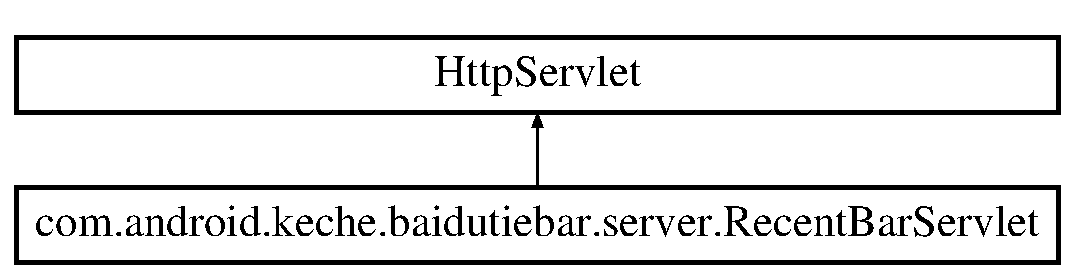
\includegraphics[height=2.000000cm]{classcom_1_1android_1_1keche_1_1baidutiebar_1_1server_1_1_recent_bar_servlet}
\end{center}
\end{figure}
\subsection*{Public 成员函数}
\begin{DoxyCompactItemize}
\item 
\mbox{\hyperlink{classcom_1_1android_1_1keche_1_1baidutiebar_1_1server_1_1_recent_bar_servlet_a1cbafb99a23906d69068f53db955898c}{Recent\+Bar\+Servlet}} ()
\end{DoxyCompactItemize}
\subsection*{Protected 成员函数}
\begin{DoxyCompactItemize}
\item 
void \mbox{\hyperlink{classcom_1_1android_1_1keche_1_1baidutiebar_1_1server_1_1_recent_bar_servlet_ae5e224734b12a10aa8f0a0936232c1b8}{do\+Get}} (Http\+Servlet\+Request request, Http\+Servlet\+Response response)  throws Servlet\+Exception, I\+O\+Exception 
\item 
void \mbox{\hyperlink{classcom_1_1android_1_1keche_1_1baidutiebar_1_1server_1_1_recent_bar_servlet_a0cbc22d0c2a7d89228df63a609b2698e}{do\+Post}} (Http\+Servlet\+Request request, Http\+Servlet\+Response response)  throws Servlet\+Exception, I\+O\+Exception 
\end{DoxyCompactItemize}


\subsection{详细描述}
Servlet implementation class \mbox{\hyperlink{classcom_1_1android_1_1keche_1_1baidutiebar_1_1server_1_1_recent_bar_servlet}{Recent\+Bar\+Servlet}} 

\subsection{构造及析构函数说明}
\mbox{\Hypertarget{classcom_1_1android_1_1keche_1_1baidutiebar_1_1server_1_1_recent_bar_servlet_a1cbafb99a23906d69068f53db955898c}\label{classcom_1_1android_1_1keche_1_1baidutiebar_1_1server_1_1_recent_bar_servlet_a1cbafb99a23906d69068f53db955898c}} 
\index{com\+::android\+::keche\+::baidutiebar\+::server\+::\+Recent\+Bar\+Servlet@{com\+::android\+::keche\+::baidutiebar\+::server\+::\+Recent\+Bar\+Servlet}!Recent\+Bar\+Servlet@{Recent\+Bar\+Servlet}}
\index{Recent\+Bar\+Servlet@{Recent\+Bar\+Servlet}!com\+::android\+::keche\+::baidutiebar\+::server\+::\+Recent\+Bar\+Servlet@{com\+::android\+::keche\+::baidutiebar\+::server\+::\+Recent\+Bar\+Servlet}}
\subsubsection{\texorpdfstring{Recent\+Bar\+Servlet()}{RecentBarServlet()}}
{\footnotesize\ttfamily com.\+android.\+keche.\+baidutiebar.\+server.\+Recent\+Bar\+Servlet.\+Recent\+Bar\+Servlet (\begin{DoxyParamCaption}{ }\end{DoxyParamCaption})\hspace{0.3cm}{\ttfamily [inline]}}

\begin{DoxySeeAlso}{参见}
Http\+Servlet\+::\+Http\+Servlet() 
\end{DoxySeeAlso}


\subsection{成员函数说明}
\mbox{\Hypertarget{classcom_1_1android_1_1keche_1_1baidutiebar_1_1server_1_1_recent_bar_servlet_ae5e224734b12a10aa8f0a0936232c1b8}\label{classcom_1_1android_1_1keche_1_1baidutiebar_1_1server_1_1_recent_bar_servlet_ae5e224734b12a10aa8f0a0936232c1b8}} 
\index{com\+::android\+::keche\+::baidutiebar\+::server\+::\+Recent\+Bar\+Servlet@{com\+::android\+::keche\+::baidutiebar\+::server\+::\+Recent\+Bar\+Servlet}!do\+Get@{do\+Get}}
\index{do\+Get@{do\+Get}!com\+::android\+::keche\+::baidutiebar\+::server\+::\+Recent\+Bar\+Servlet@{com\+::android\+::keche\+::baidutiebar\+::server\+::\+Recent\+Bar\+Servlet}}
\subsubsection{\texorpdfstring{do\+Get()}{doGet()}}
{\footnotesize\ttfamily void com.\+android.\+keche.\+baidutiebar.\+server.\+Recent\+Bar\+Servlet.\+do\+Get (\begin{DoxyParamCaption}\item[{Http\+Servlet\+Request}]{request,  }\item[{Http\+Servlet\+Response}]{response }\end{DoxyParamCaption}) throws Servlet\+Exception, I\+O\+Exception\hspace{0.3cm}{\ttfamily [inline]}, {\ttfamily [protected]}}

\begin{DoxySeeAlso}{参见}
Http\+Servlet\+::do\+Get(\+Http\+Servlet\+Request request, Http\+Servlet\+Response response) 
\end{DoxySeeAlso}
\mbox{\Hypertarget{classcom_1_1android_1_1keche_1_1baidutiebar_1_1server_1_1_recent_bar_servlet_a0cbc22d0c2a7d89228df63a609b2698e}\label{classcom_1_1android_1_1keche_1_1baidutiebar_1_1server_1_1_recent_bar_servlet_a0cbc22d0c2a7d89228df63a609b2698e}} 
\index{com\+::android\+::keche\+::baidutiebar\+::server\+::\+Recent\+Bar\+Servlet@{com\+::android\+::keche\+::baidutiebar\+::server\+::\+Recent\+Bar\+Servlet}!do\+Post@{do\+Post}}
\index{do\+Post@{do\+Post}!com\+::android\+::keche\+::baidutiebar\+::server\+::\+Recent\+Bar\+Servlet@{com\+::android\+::keche\+::baidutiebar\+::server\+::\+Recent\+Bar\+Servlet}}
\subsubsection{\texorpdfstring{do\+Post()}{doPost()}}
{\footnotesize\ttfamily void com.\+android.\+keche.\+baidutiebar.\+server.\+Recent\+Bar\+Servlet.\+do\+Post (\begin{DoxyParamCaption}\item[{Http\+Servlet\+Request}]{request,  }\item[{Http\+Servlet\+Response}]{response }\end{DoxyParamCaption}) throws Servlet\+Exception, I\+O\+Exception\hspace{0.3cm}{\ttfamily [inline]}, {\ttfamily [protected]}}

\begin{DoxySeeAlso}{参见}
Http\+Servlet\+::do\+Post(\+Http\+Servlet\+Request request, Http\+Servlet\+Response response) 
\end{DoxySeeAlso}


该类的文档由以下文件生成\+:\begin{DoxyCompactItemize}
\item 
src/com/android/keche/baidutiebar/server/Recent\+Bar\+Servlet.\+java\end{DoxyCompactItemize}

\hypertarget{classcom_1_1android_1_1keche_1_1baidutiebar_1_1server_1_1_sheet_image_servlet}{}\section{com.\+android.\+keche.\+baidutiebar.\+server.\+Sheet\+Image\+Servlet类 参考}
\label{classcom_1_1android_1_1keche_1_1baidutiebar_1_1server_1_1_sheet_image_servlet}\index{com.\+android.\+keche.\+baidutiebar.\+server.\+Sheet\+Image\+Servlet@{com.\+android.\+keche.\+baidutiebar.\+server.\+Sheet\+Image\+Servlet}}
类 com.\+android.\+keche.\+baidutiebar.\+server.\+Sheet\+Image\+Servlet 继承关系图\+:\begin{figure}[H]
\begin{center}
\leavevmode
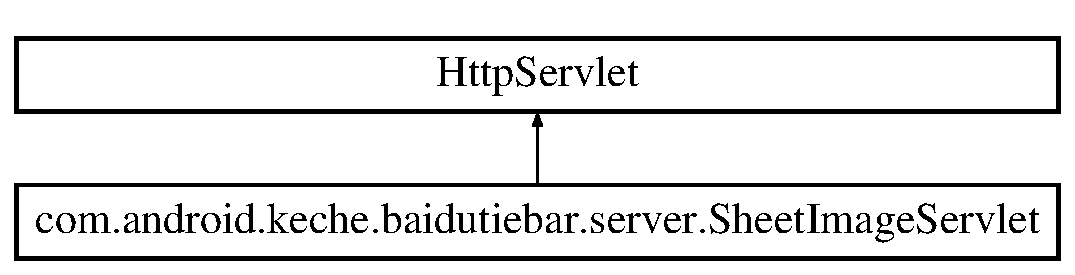
\includegraphics[height=2.000000cm]{classcom_1_1android_1_1keche_1_1baidutiebar_1_1server_1_1_sheet_image_servlet}
\end{center}
\end{figure}
\subsection*{Public 成员函数}
\begin{DoxyCompactItemize}
\item 
\mbox{\hyperlink{classcom_1_1android_1_1keche_1_1baidutiebar_1_1server_1_1_sheet_image_servlet_a52aa8341c84e9124a61a5b8d89204e7b}{Sheet\+Image\+Servlet}} ()
\end{DoxyCompactItemize}
\subsection*{Protected 成员函数}
\begin{DoxyCompactItemize}
\item 
void \mbox{\hyperlink{classcom_1_1android_1_1keche_1_1baidutiebar_1_1server_1_1_sheet_image_servlet_a09e52cc17a77d0c96845f1d9342f0f02}{do\+Get}} (Http\+Servlet\+Request request, Http\+Servlet\+Response response)  throws Servlet\+Exception, I\+O\+Exception 
\item 
void \mbox{\hyperlink{classcom_1_1android_1_1keche_1_1baidutiebar_1_1server_1_1_sheet_image_servlet_af1fb2138384d4741e045a925abfa59e4}{do\+Post}} (Http\+Servlet\+Request request, Http\+Servlet\+Response response)  throws Servlet\+Exception, I\+O\+Exception 
\end{DoxyCompactItemize}


\subsection{详细描述}
Servlet implementation class \mbox{\hyperlink{classcom_1_1android_1_1keche_1_1baidutiebar_1_1server_1_1_uploads_servlet}{Uploads\+Servlet}} 

\subsection{构造及析构函数说明}
\mbox{\Hypertarget{classcom_1_1android_1_1keche_1_1baidutiebar_1_1server_1_1_sheet_image_servlet_a52aa8341c84e9124a61a5b8d89204e7b}\label{classcom_1_1android_1_1keche_1_1baidutiebar_1_1server_1_1_sheet_image_servlet_a52aa8341c84e9124a61a5b8d89204e7b}} 
\index{com\+::android\+::keche\+::baidutiebar\+::server\+::\+Sheet\+Image\+Servlet@{com\+::android\+::keche\+::baidutiebar\+::server\+::\+Sheet\+Image\+Servlet}!Sheet\+Image\+Servlet@{Sheet\+Image\+Servlet}}
\index{Sheet\+Image\+Servlet@{Sheet\+Image\+Servlet}!com\+::android\+::keche\+::baidutiebar\+::server\+::\+Sheet\+Image\+Servlet@{com\+::android\+::keche\+::baidutiebar\+::server\+::\+Sheet\+Image\+Servlet}}
\subsubsection{\texorpdfstring{Sheet\+Image\+Servlet()}{SheetImageServlet()}}
{\footnotesize\ttfamily com.\+android.\+keche.\+baidutiebar.\+server.\+Sheet\+Image\+Servlet.\+Sheet\+Image\+Servlet (\begin{DoxyParamCaption}{ }\end{DoxyParamCaption})\hspace{0.3cm}{\ttfamily [inline]}}

\begin{DoxySeeAlso}{参见}
Http\+Servlet\+::\+Http\+Servlet() 
\end{DoxySeeAlso}


\subsection{成员函数说明}
\mbox{\Hypertarget{classcom_1_1android_1_1keche_1_1baidutiebar_1_1server_1_1_sheet_image_servlet_a09e52cc17a77d0c96845f1d9342f0f02}\label{classcom_1_1android_1_1keche_1_1baidutiebar_1_1server_1_1_sheet_image_servlet_a09e52cc17a77d0c96845f1d9342f0f02}} 
\index{com\+::android\+::keche\+::baidutiebar\+::server\+::\+Sheet\+Image\+Servlet@{com\+::android\+::keche\+::baidutiebar\+::server\+::\+Sheet\+Image\+Servlet}!do\+Get@{do\+Get}}
\index{do\+Get@{do\+Get}!com\+::android\+::keche\+::baidutiebar\+::server\+::\+Sheet\+Image\+Servlet@{com\+::android\+::keche\+::baidutiebar\+::server\+::\+Sheet\+Image\+Servlet}}
\subsubsection{\texorpdfstring{do\+Get()}{doGet()}}
{\footnotesize\ttfamily void com.\+android.\+keche.\+baidutiebar.\+server.\+Sheet\+Image\+Servlet.\+do\+Get (\begin{DoxyParamCaption}\item[{Http\+Servlet\+Request}]{request,  }\item[{Http\+Servlet\+Response}]{response }\end{DoxyParamCaption}) throws Servlet\+Exception, I\+O\+Exception\hspace{0.3cm}{\ttfamily [inline]}, {\ttfamily [protected]}}

\begin{DoxySeeAlso}{参见}
Http\+Servlet\+::do\+Get(\+Http\+Servlet\+Request request, Http\+Servlet\+Response response) 
\end{DoxySeeAlso}
\mbox{\Hypertarget{classcom_1_1android_1_1keche_1_1baidutiebar_1_1server_1_1_sheet_image_servlet_af1fb2138384d4741e045a925abfa59e4}\label{classcom_1_1android_1_1keche_1_1baidutiebar_1_1server_1_1_sheet_image_servlet_af1fb2138384d4741e045a925abfa59e4}} 
\index{com\+::android\+::keche\+::baidutiebar\+::server\+::\+Sheet\+Image\+Servlet@{com\+::android\+::keche\+::baidutiebar\+::server\+::\+Sheet\+Image\+Servlet}!do\+Post@{do\+Post}}
\index{do\+Post@{do\+Post}!com\+::android\+::keche\+::baidutiebar\+::server\+::\+Sheet\+Image\+Servlet@{com\+::android\+::keche\+::baidutiebar\+::server\+::\+Sheet\+Image\+Servlet}}
\subsubsection{\texorpdfstring{do\+Post()}{doPost()}}
{\footnotesize\ttfamily void com.\+android.\+keche.\+baidutiebar.\+server.\+Sheet\+Image\+Servlet.\+do\+Post (\begin{DoxyParamCaption}\item[{Http\+Servlet\+Request}]{request,  }\item[{Http\+Servlet\+Response}]{response }\end{DoxyParamCaption}) throws Servlet\+Exception, I\+O\+Exception\hspace{0.3cm}{\ttfamily [inline]}, {\ttfamily [protected]}}

\begin{DoxySeeAlso}{参见}
Http\+Servlet\+::do\+Post(\+Http\+Servlet\+Request request, Http\+Servlet\+Response response) 
\end{DoxySeeAlso}


该类的文档由以下文件生成\+:\begin{DoxyCompactItemize}
\item 
src/com/android/keche/baidutiebar/server/Sheet\+Image\+Servlet.\+java\end{DoxyCompactItemize}

\hypertarget{classcom_1_1android_1_1keche_1_1baidutiebar_1_1server_1_1bean_1_1_store_bean}{}\section{com.\+android.\+keche.\+baidutiebar.\+server.\+bean.\+Store\+Bean类 参考}
\label{classcom_1_1android_1_1keche_1_1baidutiebar_1_1server_1_1bean_1_1_store_bean}\index{com.\+android.\+keche.\+baidutiebar.\+server.\+bean.\+Store\+Bean@{com.\+android.\+keche.\+baidutiebar.\+server.\+bean.\+Store\+Bean}}
\subsection*{Public 成员函数}
\begin{DoxyCompactItemize}
\item 
\mbox{\Hypertarget{classcom_1_1android_1_1keche_1_1baidutiebar_1_1server_1_1bean_1_1_store_bean_a9c8963a67dd97a0f01f1fd76f69c33ca}\label{classcom_1_1android_1_1keche_1_1baidutiebar_1_1server_1_1bean_1_1_store_bean_a9c8963a67dd97a0f01f1fd76f69c33ca}} 
{\bfseries Store\+Bean} (String title, String source, String time)
\item 
\mbox{\Hypertarget{classcom_1_1android_1_1keche_1_1baidutiebar_1_1server_1_1bean_1_1_store_bean_a51d99b898a6c3f3e2e5875ca69d2e875}\label{classcom_1_1android_1_1keche_1_1baidutiebar_1_1server_1_1bean_1_1_store_bean_a51d99b898a6c3f3e2e5875ca69d2e875}} 
String {\bfseries get\+Title} ()
\item 
\mbox{\Hypertarget{classcom_1_1android_1_1keche_1_1baidutiebar_1_1server_1_1bean_1_1_store_bean_aa878a0ef1a3c329806b8f375ccba7c8c}\label{classcom_1_1android_1_1keche_1_1baidutiebar_1_1server_1_1bean_1_1_store_bean_aa878a0ef1a3c329806b8f375ccba7c8c}} 
void {\bfseries set\+Title} (String title)
\item 
\mbox{\Hypertarget{classcom_1_1android_1_1keche_1_1baidutiebar_1_1server_1_1bean_1_1_store_bean_ac89b3b25096b463cd6a04f32e0db4000}\label{classcom_1_1android_1_1keche_1_1baidutiebar_1_1server_1_1bean_1_1_store_bean_ac89b3b25096b463cd6a04f32e0db4000}} 
String {\bfseries get\+Source} ()
\item 
\mbox{\Hypertarget{classcom_1_1android_1_1keche_1_1baidutiebar_1_1server_1_1bean_1_1_store_bean_a69bd372c79d799fd7c4f83d63d2dcec4}\label{classcom_1_1android_1_1keche_1_1baidutiebar_1_1server_1_1bean_1_1_store_bean_a69bd372c79d799fd7c4f83d63d2dcec4}} 
void {\bfseries set\+Source} (String source)
\item 
\mbox{\Hypertarget{classcom_1_1android_1_1keche_1_1baidutiebar_1_1server_1_1bean_1_1_store_bean_ac945cf9e850c2224698fdd9a5fad0677}\label{classcom_1_1android_1_1keche_1_1baidutiebar_1_1server_1_1bean_1_1_store_bean_ac945cf9e850c2224698fdd9a5fad0677}} 
String {\bfseries get\+Time} ()
\item 
\mbox{\Hypertarget{classcom_1_1android_1_1keche_1_1baidutiebar_1_1server_1_1bean_1_1_store_bean_a75b3aded52c6719a5a08a88239dc8722}\label{classcom_1_1android_1_1keche_1_1baidutiebar_1_1server_1_1bean_1_1_store_bean_a75b3aded52c6719a5a08a88239dc8722}} 
void {\bfseries set\+Time} (String time)
\end{DoxyCompactItemize}


该类的文档由以下文件生成\+:\begin{DoxyCompactItemize}
\item 
src/com/android/keche/baidutiebar/server/bean/Store\+Bean.\+java\end{DoxyCompactItemize}

\hypertarget{classcom_1_1android_1_1keche_1_1baidutiebar_1_1server_1_1_store_servlet}{}\section{com.\+android.\+keche.\+baidutiebar.\+server.\+Store\+Servlet类 参考}
\label{classcom_1_1android_1_1keche_1_1baidutiebar_1_1server_1_1_store_servlet}\index{com.\+android.\+keche.\+baidutiebar.\+server.\+Store\+Servlet@{com.\+android.\+keche.\+baidutiebar.\+server.\+Store\+Servlet}}
类 com.\+android.\+keche.\+baidutiebar.\+server.\+Store\+Servlet 继承关系图\+:\begin{figure}[H]
\begin{center}
\leavevmode
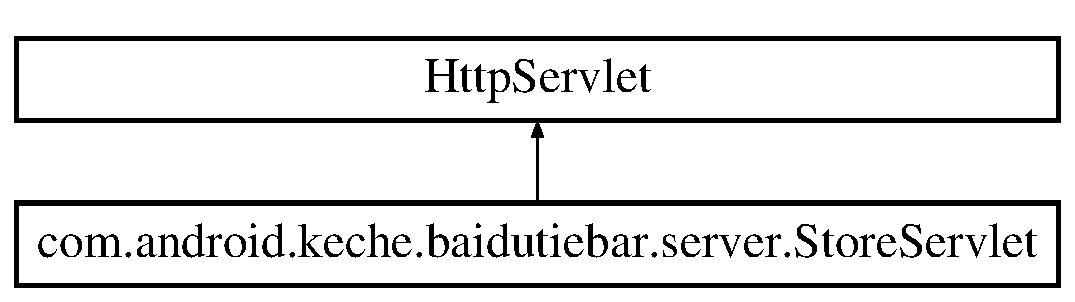
\includegraphics[height=2.000000cm]{classcom_1_1android_1_1keche_1_1baidutiebar_1_1server_1_1_store_servlet}
\end{center}
\end{figure}
\subsection*{Public 成员函数}
\begin{DoxyCompactItemize}
\item 
\mbox{\hyperlink{classcom_1_1android_1_1keche_1_1baidutiebar_1_1server_1_1_store_servlet_a672deecf5ea8ee1662bb5b6276c2efba}{Store\+Servlet}} ()
\end{DoxyCompactItemize}
\subsection*{Protected 成员函数}
\begin{DoxyCompactItemize}
\item 
void \mbox{\hyperlink{classcom_1_1android_1_1keche_1_1baidutiebar_1_1server_1_1_store_servlet_af5561d80e47cc7f9da40d6caf7d72bea}{do\+Get}} (Http\+Servlet\+Request request, Http\+Servlet\+Response response)  throws Servlet\+Exception, I\+O\+Exception 
\item 
void \mbox{\hyperlink{classcom_1_1android_1_1keche_1_1baidutiebar_1_1server_1_1_store_servlet_a033ebdbf83e2504fa7249f1ff94df27c}{do\+Post}} (Http\+Servlet\+Request request, Http\+Servlet\+Response response)  throws Servlet\+Exception, I\+O\+Exception 
\end{DoxyCompactItemize}


\subsection{详细描述}
Servlet implementation class \mbox{\hyperlink{classcom_1_1android_1_1keche_1_1baidutiebar_1_1server_1_1_store_servlet}{Store\+Servlet}} 

\subsection{构造及析构函数说明}
\mbox{\Hypertarget{classcom_1_1android_1_1keche_1_1baidutiebar_1_1server_1_1_store_servlet_a672deecf5ea8ee1662bb5b6276c2efba}\label{classcom_1_1android_1_1keche_1_1baidutiebar_1_1server_1_1_store_servlet_a672deecf5ea8ee1662bb5b6276c2efba}} 
\index{com\+::android\+::keche\+::baidutiebar\+::server\+::\+Store\+Servlet@{com\+::android\+::keche\+::baidutiebar\+::server\+::\+Store\+Servlet}!Store\+Servlet@{Store\+Servlet}}
\index{Store\+Servlet@{Store\+Servlet}!com\+::android\+::keche\+::baidutiebar\+::server\+::\+Store\+Servlet@{com\+::android\+::keche\+::baidutiebar\+::server\+::\+Store\+Servlet}}
\subsubsection{\texorpdfstring{Store\+Servlet()}{StoreServlet()}}
{\footnotesize\ttfamily com.\+android.\+keche.\+baidutiebar.\+server.\+Store\+Servlet.\+Store\+Servlet (\begin{DoxyParamCaption}{ }\end{DoxyParamCaption})\hspace{0.3cm}{\ttfamily [inline]}}

\begin{DoxySeeAlso}{参见}
Http\+Servlet\+::\+Http\+Servlet() 
\end{DoxySeeAlso}


\subsection{成员函数说明}
\mbox{\Hypertarget{classcom_1_1android_1_1keche_1_1baidutiebar_1_1server_1_1_store_servlet_af5561d80e47cc7f9da40d6caf7d72bea}\label{classcom_1_1android_1_1keche_1_1baidutiebar_1_1server_1_1_store_servlet_af5561d80e47cc7f9da40d6caf7d72bea}} 
\index{com\+::android\+::keche\+::baidutiebar\+::server\+::\+Store\+Servlet@{com\+::android\+::keche\+::baidutiebar\+::server\+::\+Store\+Servlet}!do\+Get@{do\+Get}}
\index{do\+Get@{do\+Get}!com\+::android\+::keche\+::baidutiebar\+::server\+::\+Store\+Servlet@{com\+::android\+::keche\+::baidutiebar\+::server\+::\+Store\+Servlet}}
\subsubsection{\texorpdfstring{do\+Get()}{doGet()}}
{\footnotesize\ttfamily void com.\+android.\+keche.\+baidutiebar.\+server.\+Store\+Servlet.\+do\+Get (\begin{DoxyParamCaption}\item[{Http\+Servlet\+Request}]{request,  }\item[{Http\+Servlet\+Response}]{response }\end{DoxyParamCaption}) throws Servlet\+Exception, I\+O\+Exception\hspace{0.3cm}{\ttfamily [inline]}, {\ttfamily [protected]}}

\begin{DoxySeeAlso}{参见}
Http\+Servlet\+::do\+Get(\+Http\+Servlet\+Request request, Http\+Servlet\+Response response) 
\end{DoxySeeAlso}
\mbox{\Hypertarget{classcom_1_1android_1_1keche_1_1baidutiebar_1_1server_1_1_store_servlet_a033ebdbf83e2504fa7249f1ff94df27c}\label{classcom_1_1android_1_1keche_1_1baidutiebar_1_1server_1_1_store_servlet_a033ebdbf83e2504fa7249f1ff94df27c}} 
\index{com\+::android\+::keche\+::baidutiebar\+::server\+::\+Store\+Servlet@{com\+::android\+::keche\+::baidutiebar\+::server\+::\+Store\+Servlet}!do\+Post@{do\+Post}}
\index{do\+Post@{do\+Post}!com\+::android\+::keche\+::baidutiebar\+::server\+::\+Store\+Servlet@{com\+::android\+::keche\+::baidutiebar\+::server\+::\+Store\+Servlet}}
\subsubsection{\texorpdfstring{do\+Post()}{doPost()}}
{\footnotesize\ttfamily void com.\+android.\+keche.\+baidutiebar.\+server.\+Store\+Servlet.\+do\+Post (\begin{DoxyParamCaption}\item[{Http\+Servlet\+Request}]{request,  }\item[{Http\+Servlet\+Response}]{response }\end{DoxyParamCaption}) throws Servlet\+Exception, I\+O\+Exception\hspace{0.3cm}{\ttfamily [inline]}, {\ttfamily [protected]}}

\begin{DoxySeeAlso}{参见}
Http\+Servlet\+::do\+Post(\+Http\+Servlet\+Request request, Http\+Servlet\+Response response) 
\end{DoxySeeAlso}


该类的文档由以下文件生成\+:\begin{DoxyCompactItemize}
\item 
src/com/android/keche/baidutiebar/server/Store\+Servlet.\+java\end{DoxyCompactItemize}

\hypertarget{classcom_1_1android_1_1keche_1_1baidutiebar_1_1server_1_1_uploads_servlet}{}\section{com.\+android.\+keche.\+baidutiebar.\+server.\+Uploads\+Servlet类 参考}
\label{classcom_1_1android_1_1keche_1_1baidutiebar_1_1server_1_1_uploads_servlet}\index{com.\+android.\+keche.\+baidutiebar.\+server.\+Uploads\+Servlet@{com.\+android.\+keche.\+baidutiebar.\+server.\+Uploads\+Servlet}}
类 com.\+android.\+keche.\+baidutiebar.\+server.\+Uploads\+Servlet 继承关系图\+:\begin{figure}[H]
\begin{center}
\leavevmode
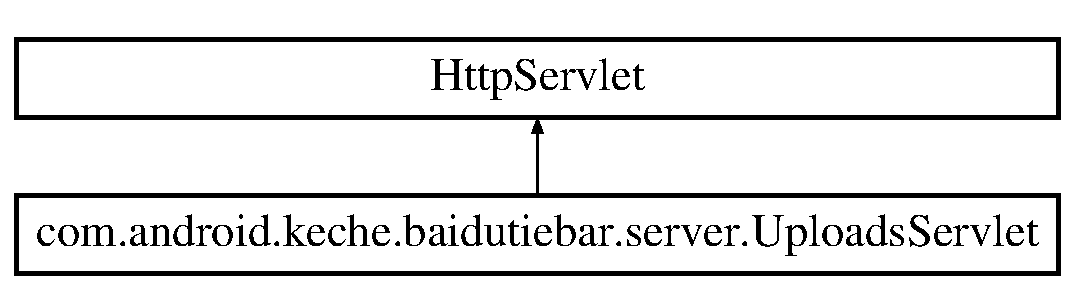
\includegraphics[height=2.000000cm]{classcom_1_1android_1_1keche_1_1baidutiebar_1_1server_1_1_uploads_servlet}
\end{center}
\end{figure}
\subsection*{Public 成员函数}
\begin{DoxyCompactItemize}
\item 
\mbox{\hyperlink{classcom_1_1android_1_1keche_1_1baidutiebar_1_1server_1_1_uploads_servlet_ab904445e2e96bb2024fe3a4acc484eb2}{Uploads\+Servlet}} ()
\end{DoxyCompactItemize}
\subsection*{Protected 成员函数}
\begin{DoxyCompactItemize}
\item 
void \mbox{\hyperlink{classcom_1_1android_1_1keche_1_1baidutiebar_1_1server_1_1_uploads_servlet_a922ca58226c6ac3ed8e3292814cb33e1}{do\+Get}} (Http\+Servlet\+Request request, Http\+Servlet\+Response response)  throws Servlet\+Exception, I\+O\+Exception 
\item 
void \mbox{\hyperlink{classcom_1_1android_1_1keche_1_1baidutiebar_1_1server_1_1_uploads_servlet_a8932c35f6e491f9b8a36f07bf494639d}{do\+Post}} (Http\+Servlet\+Request request, Http\+Servlet\+Response response)  throws Servlet\+Exception, I\+O\+Exception 
\end{DoxyCompactItemize}


\subsection{详细描述}
Servlet implementation class \mbox{\hyperlink{classcom_1_1android_1_1keche_1_1baidutiebar_1_1server_1_1_uploads_servlet}{Uploads\+Servlet}} 

\subsection{构造及析构函数说明}
\mbox{\Hypertarget{classcom_1_1android_1_1keche_1_1baidutiebar_1_1server_1_1_uploads_servlet_ab904445e2e96bb2024fe3a4acc484eb2}\label{classcom_1_1android_1_1keche_1_1baidutiebar_1_1server_1_1_uploads_servlet_ab904445e2e96bb2024fe3a4acc484eb2}} 
\index{com\+::android\+::keche\+::baidutiebar\+::server\+::\+Uploads\+Servlet@{com\+::android\+::keche\+::baidutiebar\+::server\+::\+Uploads\+Servlet}!Uploads\+Servlet@{Uploads\+Servlet}}
\index{Uploads\+Servlet@{Uploads\+Servlet}!com\+::android\+::keche\+::baidutiebar\+::server\+::\+Uploads\+Servlet@{com\+::android\+::keche\+::baidutiebar\+::server\+::\+Uploads\+Servlet}}
\subsubsection{\texorpdfstring{Uploads\+Servlet()}{UploadsServlet()}}
{\footnotesize\ttfamily com.\+android.\+keche.\+baidutiebar.\+server.\+Uploads\+Servlet.\+Uploads\+Servlet (\begin{DoxyParamCaption}{ }\end{DoxyParamCaption})\hspace{0.3cm}{\ttfamily [inline]}}

\begin{DoxySeeAlso}{参见}
Http\+Servlet\+::\+Http\+Servlet() 
\end{DoxySeeAlso}


\subsection{成员函数说明}
\mbox{\Hypertarget{classcom_1_1android_1_1keche_1_1baidutiebar_1_1server_1_1_uploads_servlet_a922ca58226c6ac3ed8e3292814cb33e1}\label{classcom_1_1android_1_1keche_1_1baidutiebar_1_1server_1_1_uploads_servlet_a922ca58226c6ac3ed8e3292814cb33e1}} 
\index{com\+::android\+::keche\+::baidutiebar\+::server\+::\+Uploads\+Servlet@{com\+::android\+::keche\+::baidutiebar\+::server\+::\+Uploads\+Servlet}!do\+Get@{do\+Get}}
\index{do\+Get@{do\+Get}!com\+::android\+::keche\+::baidutiebar\+::server\+::\+Uploads\+Servlet@{com\+::android\+::keche\+::baidutiebar\+::server\+::\+Uploads\+Servlet}}
\subsubsection{\texorpdfstring{do\+Get()}{doGet()}}
{\footnotesize\ttfamily void com.\+android.\+keche.\+baidutiebar.\+server.\+Uploads\+Servlet.\+do\+Get (\begin{DoxyParamCaption}\item[{Http\+Servlet\+Request}]{request,  }\item[{Http\+Servlet\+Response}]{response }\end{DoxyParamCaption}) throws Servlet\+Exception, I\+O\+Exception\hspace{0.3cm}{\ttfamily [inline]}, {\ttfamily [protected]}}

\begin{DoxySeeAlso}{参见}
Http\+Servlet\+::do\+Get(\+Http\+Servlet\+Request request, Http\+Servlet\+Response response) 
\end{DoxySeeAlso}
\mbox{\Hypertarget{classcom_1_1android_1_1keche_1_1baidutiebar_1_1server_1_1_uploads_servlet_a8932c35f6e491f9b8a36f07bf494639d}\label{classcom_1_1android_1_1keche_1_1baidutiebar_1_1server_1_1_uploads_servlet_a8932c35f6e491f9b8a36f07bf494639d}} 
\index{com\+::android\+::keche\+::baidutiebar\+::server\+::\+Uploads\+Servlet@{com\+::android\+::keche\+::baidutiebar\+::server\+::\+Uploads\+Servlet}!do\+Post@{do\+Post}}
\index{do\+Post@{do\+Post}!com\+::android\+::keche\+::baidutiebar\+::server\+::\+Uploads\+Servlet@{com\+::android\+::keche\+::baidutiebar\+::server\+::\+Uploads\+Servlet}}
\subsubsection{\texorpdfstring{do\+Post()}{doPost()}}
{\footnotesize\ttfamily void com.\+android.\+keche.\+baidutiebar.\+server.\+Uploads\+Servlet.\+do\+Post (\begin{DoxyParamCaption}\item[{Http\+Servlet\+Request}]{request,  }\item[{Http\+Servlet\+Response}]{response }\end{DoxyParamCaption}) throws Servlet\+Exception, I\+O\+Exception\hspace{0.3cm}{\ttfamily [inline]}, {\ttfamily [protected]}}

\begin{DoxySeeAlso}{参见}
Http\+Servlet\+::do\+Post(\+Http\+Servlet\+Request request, Http\+Servlet\+Response response) 
\end{DoxySeeAlso}


该类的文档由以下文件生成\+:\begin{DoxyCompactItemize}
\item 
src/com/android/keche/baidutiebar/server/Uploads\+Servlet.\+java\end{DoxyCompactItemize}

\hypertarget{classcom_1_1android_1_1keche_1_1baidutiebar_1_1server_1_1bean_1_1_user_ex_bean}{}\section{com.\+android.\+keche.\+baidutiebar.\+server.\+bean.\+User\+Ex\+Bean类 参考}
\label{classcom_1_1android_1_1keche_1_1baidutiebar_1_1server_1_1bean_1_1_user_ex_bean}\index{com.\+android.\+keche.\+baidutiebar.\+server.\+bean.\+User\+Ex\+Bean@{com.\+android.\+keche.\+baidutiebar.\+server.\+bean.\+User\+Ex\+Bean}}


用户类的创建、修改和查看 该类用于网络传递 是 User\+Bean的加强版  


\subsection*{Public 成员函数}
\begin{DoxyCompactItemize}
\item 
\mbox{\hyperlink{classcom_1_1android_1_1keche_1_1baidutiebar_1_1server_1_1bean_1_1_user_ex_bean_ac2fc10920dc549e182bc8e8a869f4b3b}{User\+Ex\+Bean}} (String name, String password)
\begin{DoxyCompactList}\small\item\em 用户表的构造方法 \end{DoxyCompactList}\item 
\mbox{\Hypertarget{classcom_1_1android_1_1keche_1_1baidutiebar_1_1server_1_1bean_1_1_user_ex_bean_a38594a57228bc114af5465764b915bc0}\label{classcom_1_1android_1_1keche_1_1baidutiebar_1_1server_1_1bean_1_1_user_ex_bean_a38594a57228bc114af5465764b915bc0}} 
{\bfseries User\+Ex\+Bean} (String name, String password, String icon\+String, int fans\+Num, int focus\+Num)
\item 
\mbox{\Hypertarget{classcom_1_1android_1_1keche_1_1baidutiebar_1_1server_1_1bean_1_1_user_ex_bean_a02851cd0139adc51845db349ac40490e}\label{classcom_1_1android_1_1keche_1_1baidutiebar_1_1server_1_1bean_1_1_user_ex_bean_a02851cd0139adc51845db349ac40490e}} 
int {\bfseries get\+Id} ()
\item 
\mbox{\Hypertarget{classcom_1_1android_1_1keche_1_1baidutiebar_1_1server_1_1bean_1_1_user_ex_bean_a982cefa310d5429c44029dbcb8560acc}\label{classcom_1_1android_1_1keche_1_1baidutiebar_1_1server_1_1bean_1_1_user_ex_bean_a982cefa310d5429c44029dbcb8560acc}} 
void {\bfseries set\+Id} (int id)
\item 
String \mbox{\hyperlink{classcom_1_1android_1_1keche_1_1baidutiebar_1_1server_1_1bean_1_1_user_ex_bean_ac1bf507f7cc774d41c89d117f23176c5}{get\+Name}} ()
\item 
void \mbox{\hyperlink{classcom_1_1android_1_1keche_1_1baidutiebar_1_1server_1_1bean_1_1_user_ex_bean_a9253999f7ad946c03a3a7e1fd88fdfdd}{set\+Name}} (String name)
\item 
String \mbox{\hyperlink{classcom_1_1android_1_1keche_1_1baidutiebar_1_1server_1_1bean_1_1_user_ex_bean_acc2bcd547a37930973ecf55395970b46}{get\+Password}} ()
\item 
void \mbox{\hyperlink{classcom_1_1android_1_1keche_1_1baidutiebar_1_1server_1_1bean_1_1_user_ex_bean_a1322157e2aa219a479385d48ae594e15}{set\+Password}} (String password)
\item 
\mbox{\Hypertarget{classcom_1_1android_1_1keche_1_1baidutiebar_1_1server_1_1bean_1_1_user_ex_bean_ae19916e627a1577391b4a246124bb827}\label{classcom_1_1android_1_1keche_1_1baidutiebar_1_1server_1_1bean_1_1_user_ex_bean_ae19916e627a1577391b4a246124bb827}} 
String {\bfseries get\+Icon\+Url} ()
\item 
\mbox{\Hypertarget{classcom_1_1android_1_1keche_1_1baidutiebar_1_1server_1_1bean_1_1_user_ex_bean_a2f5a8c4fcb7b9d40d8ab71acc5368873}\label{classcom_1_1android_1_1keche_1_1baidutiebar_1_1server_1_1bean_1_1_user_ex_bean_a2f5a8c4fcb7b9d40d8ab71acc5368873}} 
void {\bfseries set\+Icon\+Url} (String icon\+String)
\item 
\mbox{\Hypertarget{classcom_1_1android_1_1keche_1_1baidutiebar_1_1server_1_1bean_1_1_user_ex_bean_a93ac14a244d09b6117e0b69b7c7b89f6}\label{classcom_1_1android_1_1keche_1_1baidutiebar_1_1server_1_1bean_1_1_user_ex_bean_a93ac14a244d09b6117e0b69b7c7b89f6}} 
String {\bfseries get\+Old} ()
\item 
\mbox{\Hypertarget{classcom_1_1android_1_1keche_1_1baidutiebar_1_1server_1_1bean_1_1_user_ex_bean_ad2b2cdb2769b1c944a266b55b707270c}\label{classcom_1_1android_1_1keche_1_1baidutiebar_1_1server_1_1bean_1_1_user_ex_bean_ad2b2cdb2769b1c944a266b55b707270c}} 
void {\bfseries set\+Old} (String old)
\item 
\mbox{\Hypertarget{classcom_1_1android_1_1keche_1_1baidutiebar_1_1server_1_1bean_1_1_user_ex_bean_a2923e552d4ae08115f5cc9cd58bfeff3}\label{classcom_1_1android_1_1keche_1_1baidutiebar_1_1server_1_1bean_1_1_user_ex_bean_a2923e552d4ae08115f5cc9cd58bfeff3}} 
int {\bfseries get\+Fans\+Num} ()
\item 
\mbox{\Hypertarget{classcom_1_1android_1_1keche_1_1baidutiebar_1_1server_1_1bean_1_1_user_ex_bean_aa2fc68dd8549becc82898dbf334b133e}\label{classcom_1_1android_1_1keche_1_1baidutiebar_1_1server_1_1bean_1_1_user_ex_bean_aa2fc68dd8549becc82898dbf334b133e}} 
void {\bfseries set\+Fans\+Num} (int fans\+Num)
\item 
\mbox{\Hypertarget{classcom_1_1android_1_1keche_1_1baidutiebar_1_1server_1_1bean_1_1_user_ex_bean_a7abe6f3f26f76affedd55ca0968220f1}\label{classcom_1_1android_1_1keche_1_1baidutiebar_1_1server_1_1bean_1_1_user_ex_bean_a7abe6f3f26f76affedd55ca0968220f1}} 
int {\bfseries get\+Focus\+Num} ()
\item 
\mbox{\Hypertarget{classcom_1_1android_1_1keche_1_1baidutiebar_1_1server_1_1bean_1_1_user_ex_bean_a111516621e6d40fb3a34bf7c16cc98e0}\label{classcom_1_1android_1_1keche_1_1baidutiebar_1_1server_1_1bean_1_1_user_ex_bean_a111516621e6d40fb3a34bf7c16cc98e0}} 
void {\bfseries set\+Focus\+Num} (int focus\+Num)
\item 
String \mbox{\hyperlink{classcom_1_1android_1_1keche_1_1baidutiebar_1_1server_1_1bean_1_1_user_ex_bean_a126aaffad5bf9514c6d3df91a440f683}{to\+String}} ()
\end{DoxyCompactItemize}


\subsection{详细描述}
用户类的创建、修改和查看 该类用于网络传递 是 User\+Bean的加强版 

\begin{DoxyAuthor}{作者}
马宏涛 
\end{DoxyAuthor}


\subsection{构造及析构函数说明}
\mbox{\Hypertarget{classcom_1_1android_1_1keche_1_1baidutiebar_1_1server_1_1bean_1_1_user_ex_bean_ac2fc10920dc549e182bc8e8a869f4b3b}\label{classcom_1_1android_1_1keche_1_1baidutiebar_1_1server_1_1bean_1_1_user_ex_bean_ac2fc10920dc549e182bc8e8a869f4b3b}} 
\index{com\+::android\+::keche\+::baidutiebar\+::server\+::bean\+::\+User\+Ex\+Bean@{com\+::android\+::keche\+::baidutiebar\+::server\+::bean\+::\+User\+Ex\+Bean}!User\+Ex\+Bean@{User\+Ex\+Bean}}
\index{User\+Ex\+Bean@{User\+Ex\+Bean}!com\+::android\+::keche\+::baidutiebar\+::server\+::bean\+::\+User\+Ex\+Bean@{com\+::android\+::keche\+::baidutiebar\+::server\+::bean\+::\+User\+Ex\+Bean}}
\subsubsection{\texorpdfstring{User\+Ex\+Bean()}{UserExBean()}}
{\footnotesize\ttfamily com.\+android.\+keche.\+baidutiebar.\+server.\+bean.\+User\+Ex\+Bean.\+User\+Ex\+Bean (\begin{DoxyParamCaption}\item[{String}]{name,  }\item[{String}]{password }\end{DoxyParamCaption})\hspace{0.3cm}{\ttfamily [inline]}}



用户表的构造方法 


\begin{DoxyParams}{参数}
{\em name} & 用户名 \\
\hline
{\em password} & 密码 \\
\hline
\end{DoxyParams}


\subsection{成员函数说明}
\mbox{\Hypertarget{classcom_1_1android_1_1keche_1_1baidutiebar_1_1server_1_1bean_1_1_user_ex_bean_ac1bf507f7cc774d41c89d117f23176c5}\label{classcom_1_1android_1_1keche_1_1baidutiebar_1_1server_1_1bean_1_1_user_ex_bean_ac1bf507f7cc774d41c89d117f23176c5}} 
\index{com\+::android\+::keche\+::baidutiebar\+::server\+::bean\+::\+User\+Ex\+Bean@{com\+::android\+::keche\+::baidutiebar\+::server\+::bean\+::\+User\+Ex\+Bean}!get\+Name@{get\+Name}}
\index{get\+Name@{get\+Name}!com\+::android\+::keche\+::baidutiebar\+::server\+::bean\+::\+User\+Ex\+Bean@{com\+::android\+::keche\+::baidutiebar\+::server\+::bean\+::\+User\+Ex\+Bean}}
\subsubsection{\texorpdfstring{get\+Name()}{getName()}}
{\footnotesize\ttfamily String com.\+android.\+keche.\+baidutiebar.\+server.\+bean.\+User\+Ex\+Bean.\+get\+Name (\begin{DoxyParamCaption}{ }\end{DoxyParamCaption})\hspace{0.3cm}{\ttfamily [inline]}}

返回用户名 \begin{DoxyReturn}{返回}
用户名 
\end{DoxyReturn}
\mbox{\Hypertarget{classcom_1_1android_1_1keche_1_1baidutiebar_1_1server_1_1bean_1_1_user_ex_bean_acc2bcd547a37930973ecf55395970b46}\label{classcom_1_1android_1_1keche_1_1baidutiebar_1_1server_1_1bean_1_1_user_ex_bean_acc2bcd547a37930973ecf55395970b46}} 
\index{com\+::android\+::keche\+::baidutiebar\+::server\+::bean\+::\+User\+Ex\+Bean@{com\+::android\+::keche\+::baidutiebar\+::server\+::bean\+::\+User\+Ex\+Bean}!get\+Password@{get\+Password}}
\index{get\+Password@{get\+Password}!com\+::android\+::keche\+::baidutiebar\+::server\+::bean\+::\+User\+Ex\+Bean@{com\+::android\+::keche\+::baidutiebar\+::server\+::bean\+::\+User\+Ex\+Bean}}
\subsubsection{\texorpdfstring{get\+Password()}{getPassword()}}
{\footnotesize\ttfamily String com.\+android.\+keche.\+baidutiebar.\+server.\+bean.\+User\+Ex\+Bean.\+get\+Password (\begin{DoxyParamCaption}{ }\end{DoxyParamCaption})\hspace{0.3cm}{\ttfamily [inline]}}

返回密码 \begin{DoxyReturn}{返回}
密码 
\end{DoxyReturn}
\mbox{\Hypertarget{classcom_1_1android_1_1keche_1_1baidutiebar_1_1server_1_1bean_1_1_user_ex_bean_a9253999f7ad946c03a3a7e1fd88fdfdd}\label{classcom_1_1android_1_1keche_1_1baidutiebar_1_1server_1_1bean_1_1_user_ex_bean_a9253999f7ad946c03a3a7e1fd88fdfdd}} 
\index{com\+::android\+::keche\+::baidutiebar\+::server\+::bean\+::\+User\+Ex\+Bean@{com\+::android\+::keche\+::baidutiebar\+::server\+::bean\+::\+User\+Ex\+Bean}!set\+Name@{set\+Name}}
\index{set\+Name@{set\+Name}!com\+::android\+::keche\+::baidutiebar\+::server\+::bean\+::\+User\+Ex\+Bean@{com\+::android\+::keche\+::baidutiebar\+::server\+::bean\+::\+User\+Ex\+Bean}}
\subsubsection{\texorpdfstring{set\+Name()}{setName()}}
{\footnotesize\ttfamily void com.\+android.\+keche.\+baidutiebar.\+server.\+bean.\+User\+Ex\+Bean.\+set\+Name (\begin{DoxyParamCaption}\item[{String}]{name }\end{DoxyParamCaption})\hspace{0.3cm}{\ttfamily [inline]}}

设置用户名 
\begin{DoxyParams}{参数}
{\em name} & 用户名 \\
\hline
\end{DoxyParams}
\mbox{\Hypertarget{classcom_1_1android_1_1keche_1_1baidutiebar_1_1server_1_1bean_1_1_user_ex_bean_a1322157e2aa219a479385d48ae594e15}\label{classcom_1_1android_1_1keche_1_1baidutiebar_1_1server_1_1bean_1_1_user_ex_bean_a1322157e2aa219a479385d48ae594e15}} 
\index{com\+::android\+::keche\+::baidutiebar\+::server\+::bean\+::\+User\+Ex\+Bean@{com\+::android\+::keche\+::baidutiebar\+::server\+::bean\+::\+User\+Ex\+Bean}!set\+Password@{set\+Password}}
\index{set\+Password@{set\+Password}!com\+::android\+::keche\+::baidutiebar\+::server\+::bean\+::\+User\+Ex\+Bean@{com\+::android\+::keche\+::baidutiebar\+::server\+::bean\+::\+User\+Ex\+Bean}}
\subsubsection{\texorpdfstring{set\+Password()}{setPassword()}}
{\footnotesize\ttfamily void com.\+android.\+keche.\+baidutiebar.\+server.\+bean.\+User\+Ex\+Bean.\+set\+Password (\begin{DoxyParamCaption}\item[{String}]{password }\end{DoxyParamCaption})\hspace{0.3cm}{\ttfamily [inline]}}

设置密码 
\begin{DoxyParams}{参数}
{\em password} & 密码 \\
\hline
\end{DoxyParams}
\mbox{\Hypertarget{classcom_1_1android_1_1keche_1_1baidutiebar_1_1server_1_1bean_1_1_user_ex_bean_a126aaffad5bf9514c6d3df91a440f683}\label{classcom_1_1android_1_1keche_1_1baidutiebar_1_1server_1_1bean_1_1_user_ex_bean_a126aaffad5bf9514c6d3df91a440f683}} 
\index{com\+::android\+::keche\+::baidutiebar\+::server\+::bean\+::\+User\+Ex\+Bean@{com\+::android\+::keche\+::baidutiebar\+::server\+::bean\+::\+User\+Ex\+Bean}!to\+String@{to\+String}}
\index{to\+String@{to\+String}!com\+::android\+::keche\+::baidutiebar\+::server\+::bean\+::\+User\+Ex\+Bean@{com\+::android\+::keche\+::baidutiebar\+::server\+::bean\+::\+User\+Ex\+Bean}}
\subsubsection{\texorpdfstring{to\+String()}{toString()}}
{\footnotesize\ttfamily String com.\+android.\+keche.\+baidutiebar.\+server.\+bean.\+User\+Ex\+Bean.\+to\+String (\begin{DoxyParamCaption}{ }\end{DoxyParamCaption})\hspace{0.3cm}{\ttfamily [inline]}}

读取用户表 \begin{DoxyReturn}{返回}
用户名密码 
\end{DoxyReturn}


该类的文档由以下文件生成\+:\begin{DoxyCompactItemize}
\item 
src/com/android/keche/baidutiebar/server/bean/User\+Ex\+Bean.\+java\end{DoxyCompactItemize}

\hypertarget{classcom_1_1android_1_1keche_1_1baidutiebar_1_1server_1_1_user_icon_servlet}{}\section{com.\+android.\+keche.\+baidutiebar.\+server.\+User\+Icon\+Servlet类 参考}
\label{classcom_1_1android_1_1keche_1_1baidutiebar_1_1server_1_1_user_icon_servlet}\index{com.\+android.\+keche.\+baidutiebar.\+server.\+User\+Icon\+Servlet@{com.\+android.\+keche.\+baidutiebar.\+server.\+User\+Icon\+Servlet}}
类 com.\+android.\+keche.\+baidutiebar.\+server.\+User\+Icon\+Servlet 继承关系图\+:\begin{figure}[H]
\begin{center}
\leavevmode
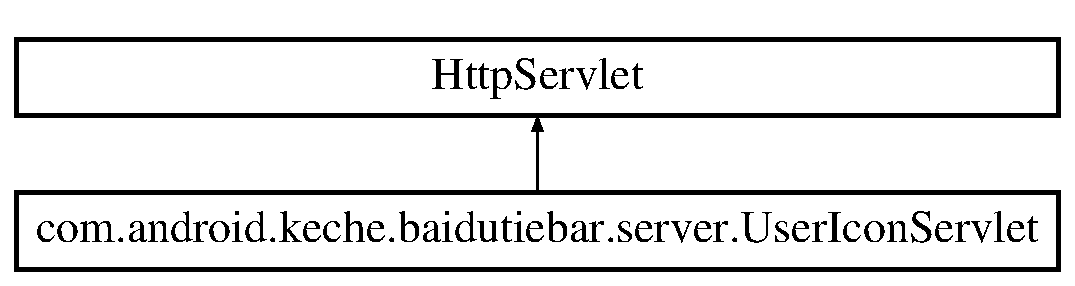
\includegraphics[height=2.000000cm]{classcom_1_1android_1_1keche_1_1baidutiebar_1_1server_1_1_user_icon_servlet}
\end{center}
\end{figure}
\subsection*{Public 成员函数}
\begin{DoxyCompactItemize}
\item 
\mbox{\hyperlink{classcom_1_1android_1_1keche_1_1baidutiebar_1_1server_1_1_user_icon_servlet_aca4f4626a8e20be6168698449bd89c0c}{User\+Icon\+Servlet}} ()
\end{DoxyCompactItemize}
\subsection*{Protected 成员函数}
\begin{DoxyCompactItemize}
\item 
void \mbox{\hyperlink{classcom_1_1android_1_1keche_1_1baidutiebar_1_1server_1_1_user_icon_servlet_a920f6cc5672eeb21bf765fce8b7396aa}{do\+Get}} (Http\+Servlet\+Request request, Http\+Servlet\+Response response)  throws Servlet\+Exception, I\+O\+Exception 
\item 
void \mbox{\hyperlink{classcom_1_1android_1_1keche_1_1baidutiebar_1_1server_1_1_user_icon_servlet_abceadf7e5eb5fde6a29a142e59f21616}{do\+Post}} (Http\+Servlet\+Request request, Http\+Servlet\+Response response)  throws Servlet\+Exception, I\+O\+Exception 
\end{DoxyCompactItemize}


\subsection{详细描述}
Servlet implementation class \mbox{\hyperlink{classcom_1_1android_1_1keche_1_1baidutiebar_1_1server_1_1_uploads_servlet}{Uploads\+Servlet}} 

\subsection{构造及析构函数说明}
\mbox{\Hypertarget{classcom_1_1android_1_1keche_1_1baidutiebar_1_1server_1_1_user_icon_servlet_aca4f4626a8e20be6168698449bd89c0c}\label{classcom_1_1android_1_1keche_1_1baidutiebar_1_1server_1_1_user_icon_servlet_aca4f4626a8e20be6168698449bd89c0c}} 
\index{com\+::android\+::keche\+::baidutiebar\+::server\+::\+User\+Icon\+Servlet@{com\+::android\+::keche\+::baidutiebar\+::server\+::\+User\+Icon\+Servlet}!User\+Icon\+Servlet@{User\+Icon\+Servlet}}
\index{User\+Icon\+Servlet@{User\+Icon\+Servlet}!com\+::android\+::keche\+::baidutiebar\+::server\+::\+User\+Icon\+Servlet@{com\+::android\+::keche\+::baidutiebar\+::server\+::\+User\+Icon\+Servlet}}
\subsubsection{\texorpdfstring{User\+Icon\+Servlet()}{UserIconServlet()}}
{\footnotesize\ttfamily com.\+android.\+keche.\+baidutiebar.\+server.\+User\+Icon\+Servlet.\+User\+Icon\+Servlet (\begin{DoxyParamCaption}{ }\end{DoxyParamCaption})\hspace{0.3cm}{\ttfamily [inline]}}

\begin{DoxySeeAlso}{参见}
Http\+Servlet\+::\+Http\+Servlet() 
\end{DoxySeeAlso}


\subsection{成员函数说明}
\mbox{\Hypertarget{classcom_1_1android_1_1keche_1_1baidutiebar_1_1server_1_1_user_icon_servlet_a920f6cc5672eeb21bf765fce8b7396aa}\label{classcom_1_1android_1_1keche_1_1baidutiebar_1_1server_1_1_user_icon_servlet_a920f6cc5672eeb21bf765fce8b7396aa}} 
\index{com\+::android\+::keche\+::baidutiebar\+::server\+::\+User\+Icon\+Servlet@{com\+::android\+::keche\+::baidutiebar\+::server\+::\+User\+Icon\+Servlet}!do\+Get@{do\+Get}}
\index{do\+Get@{do\+Get}!com\+::android\+::keche\+::baidutiebar\+::server\+::\+User\+Icon\+Servlet@{com\+::android\+::keche\+::baidutiebar\+::server\+::\+User\+Icon\+Servlet}}
\subsubsection{\texorpdfstring{do\+Get()}{doGet()}}
{\footnotesize\ttfamily void com.\+android.\+keche.\+baidutiebar.\+server.\+User\+Icon\+Servlet.\+do\+Get (\begin{DoxyParamCaption}\item[{Http\+Servlet\+Request}]{request,  }\item[{Http\+Servlet\+Response}]{response }\end{DoxyParamCaption}) throws Servlet\+Exception, I\+O\+Exception\hspace{0.3cm}{\ttfamily [inline]}, {\ttfamily [protected]}}

\begin{DoxySeeAlso}{参见}
Http\+Servlet\+::do\+Get(\+Http\+Servlet\+Request request, Http\+Servlet\+Response response) 
\end{DoxySeeAlso}
\mbox{\Hypertarget{classcom_1_1android_1_1keche_1_1baidutiebar_1_1server_1_1_user_icon_servlet_abceadf7e5eb5fde6a29a142e59f21616}\label{classcom_1_1android_1_1keche_1_1baidutiebar_1_1server_1_1_user_icon_servlet_abceadf7e5eb5fde6a29a142e59f21616}} 
\index{com\+::android\+::keche\+::baidutiebar\+::server\+::\+User\+Icon\+Servlet@{com\+::android\+::keche\+::baidutiebar\+::server\+::\+User\+Icon\+Servlet}!do\+Post@{do\+Post}}
\index{do\+Post@{do\+Post}!com\+::android\+::keche\+::baidutiebar\+::server\+::\+User\+Icon\+Servlet@{com\+::android\+::keche\+::baidutiebar\+::server\+::\+User\+Icon\+Servlet}}
\subsubsection{\texorpdfstring{do\+Post()}{doPost()}}
{\footnotesize\ttfamily void com.\+android.\+keche.\+baidutiebar.\+server.\+User\+Icon\+Servlet.\+do\+Post (\begin{DoxyParamCaption}\item[{Http\+Servlet\+Request}]{request,  }\item[{Http\+Servlet\+Response}]{response }\end{DoxyParamCaption}) throws Servlet\+Exception, I\+O\+Exception\hspace{0.3cm}{\ttfamily [inline]}, {\ttfamily [protected]}}

\begin{DoxySeeAlso}{参见}
Http\+Servlet\+::do\+Post(\+Http\+Servlet\+Request request, Http\+Servlet\+Response response) 
\end{DoxySeeAlso}


该类的文档由以下文件生成\+:\begin{DoxyCompactItemize}
\item 
src/com/android/keche/baidutiebar/server/User\+Icon\+Servlet.\+java\end{DoxyCompactItemize}

%--- End generated contents ---

% Index
\backmatter
\newpage
\phantomsection
\clearemptydoublepage
\addcontentsline{toc}{chapter}{索引}
\printindex

\end{document}
